% tisane/figures/tables to include:
% [usage scenario] 1. Overview of Tisane code, showcase all language constructs through multiple examples --> usage scenario (Pigs), appendix (Barr)
% [usage scenario] 2. Overview of disambiguation --> Pigs, Barr (random effects or family/link tabs)
% [draft] 3. Table describing clustering examples
% [] 4. Table/figure comparing existing tools with Tisane in terms of who is in charge of validity (row of checkboxes that say system does or system-human hybrid collab)
% 5. Overview of system workflow/interaction (language, representation, diambiguation, code generation, interactive compilation process is the entire thing)

%\def\myequation{$Y = \beta_{0} + \beta_{1} X_{1} + \cdots + \beta_{n} X_{n}$}

\newcommand{\figureSystemOverview}{
%    \pgfplotstableread[col sep = comma]{tisane/figures/resid_plot.csv}\loadedtable

    \begin{figure*}%[h]
        \centering
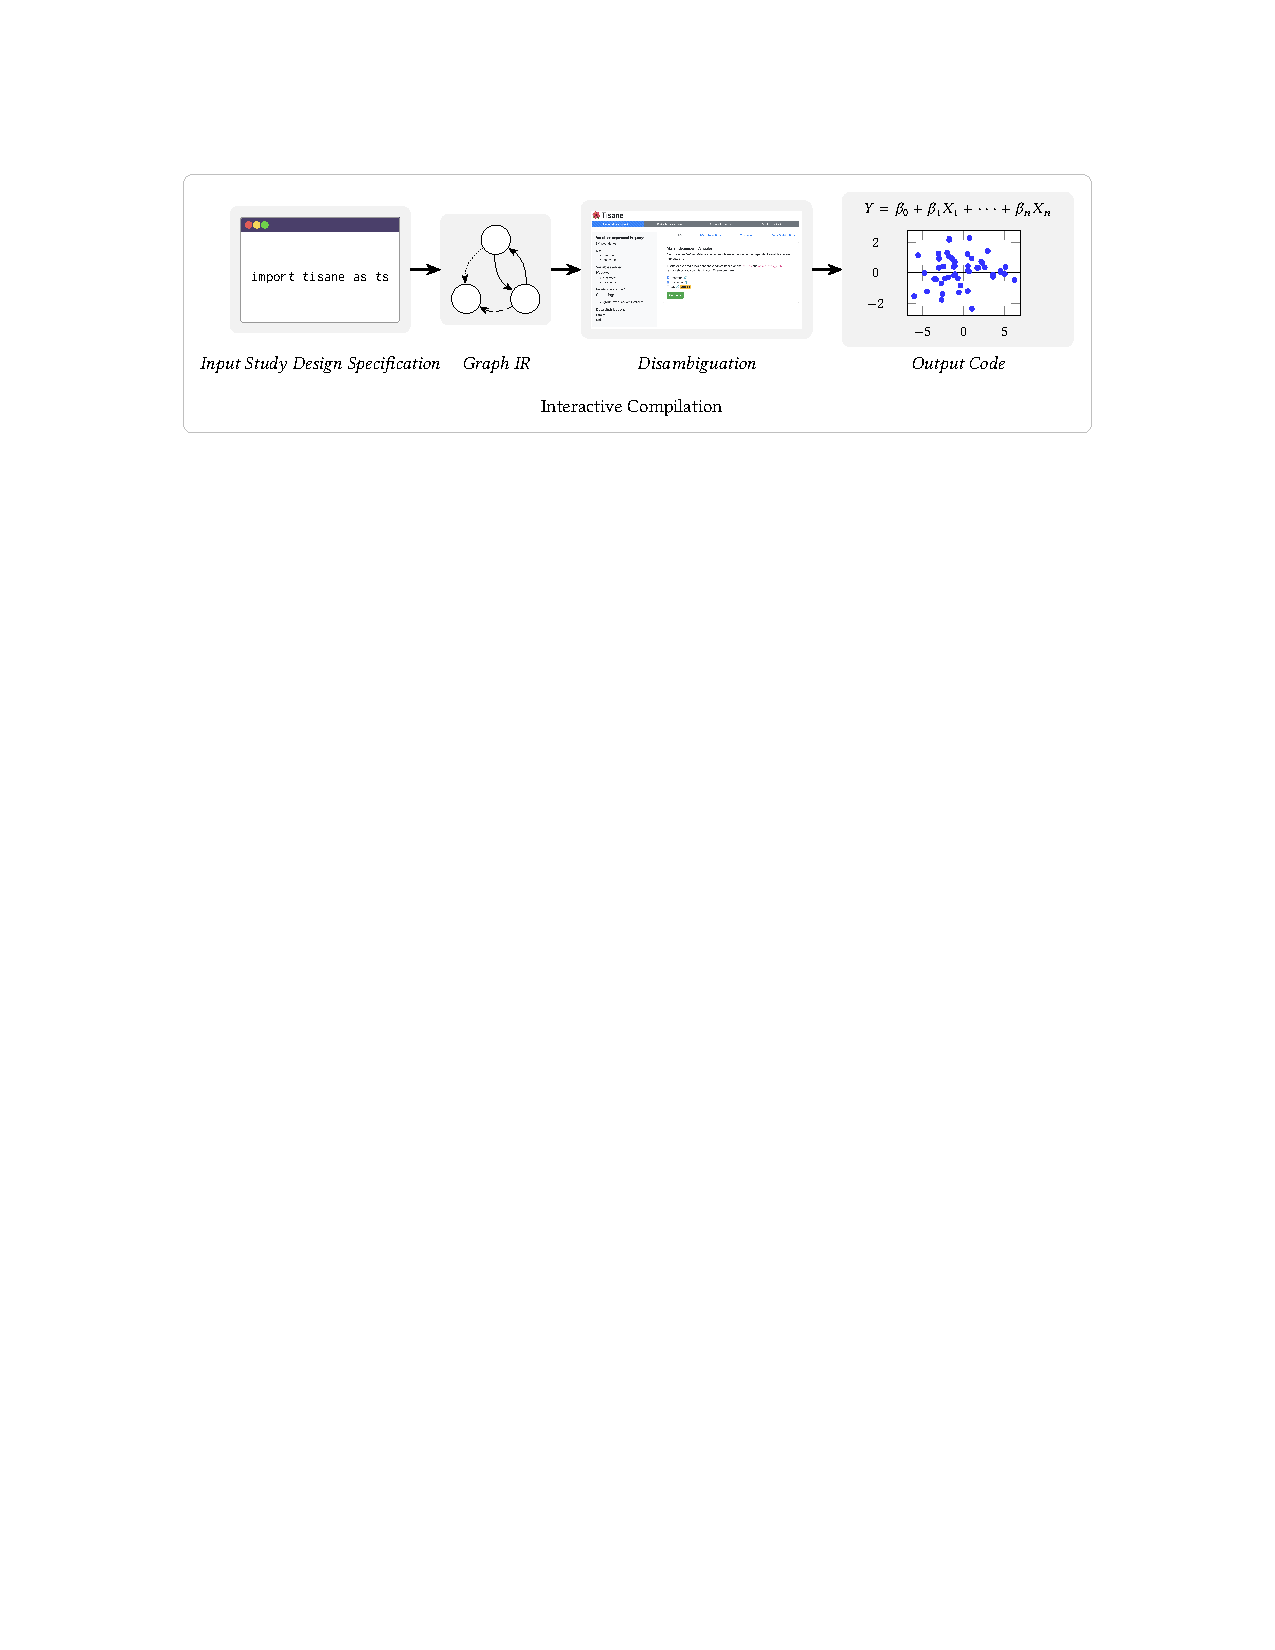
\includegraphics{tisane/figures/figure1}
%        \begin{tikzpicture}[>=Stealth,
%                            every node/.style={node distance=0.5cm}]
%            \begin{scope}[local bounding box=bb,
%                          every node/.style={inner sep=5pt, node distance=0.5cm},
%                          stage/.style={fill=gray!10,rounded corners=4pt},
%                          caption/.style={node distance=.2cm,rounded corners=4pt}]
%                % \node[stage] (input) at (0, 0) {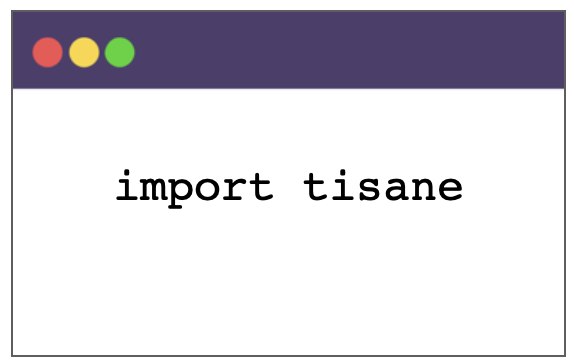
\includegraphics[width=.13\textwidth]{tisane/figures/tisane_code_icon}};
%                \node[stage] (input) at (0, 0) {\begin{tikzpicture}[every node/.style={inner sep=0pt},
%                                                                    button/.style={circle,minimum size=3pt}]
%                    \node[rectangle split, rectangle split parts=2, rounded corners=1pt, rectangle split part fill={tisanecodetop,white},rectangle split empty part height=7pt,inner sep=0pt,draw=gray!80,rectangle split draw splits=false] (n) {\nodepart{two} \begin{tikzpicture}
%                        \node[inner sep=5pt,rectangle, minimum height=1.5cm]       {\footnotesize \texttt{import tisane as ts}};
%                    \end{tikzpicture}};
%                    \coordinate (start) at ($(n.text west)+(4pt,0)$);
%                    \node[button,fill=closecolor]   (close) at (start) {};
%                    \node[button,fill=minimizecolor,right=0.5pt of close] (minimize) {};
%                    \node[button,fill=maximizecolor,right=0.5pt of minimize] (maximize) {};
%                \end{tikzpicture}};
%                % \node[caption,below=of input]   {\textit{Input Study Design specification}};
%                \node[right=of input,stage] (graphir) {\begin{tikzpicture}[every node/.style={circle, draw=black,fill=white}]
%                    \node (a) at (0,0) {};
%                    \node (b) at (-0.5, -1) {};
%                    \node (c) at (0.5, -1) {};
%                    \graph{
%                        (a) ->[densely dotted,bend right] (b);
%                        (c) ->[bend right] (a);
%                        (a) ->[bend right] (c);
%                        (c) ->[densely dashed,bend left] (b);
%                    };
%                \end{tikzpicture}};
%                % \node[caption,below=of graphir] (graphircaption) {\textit{Graph IR}};
%                \node[right=of graphir,stage] (disambig) {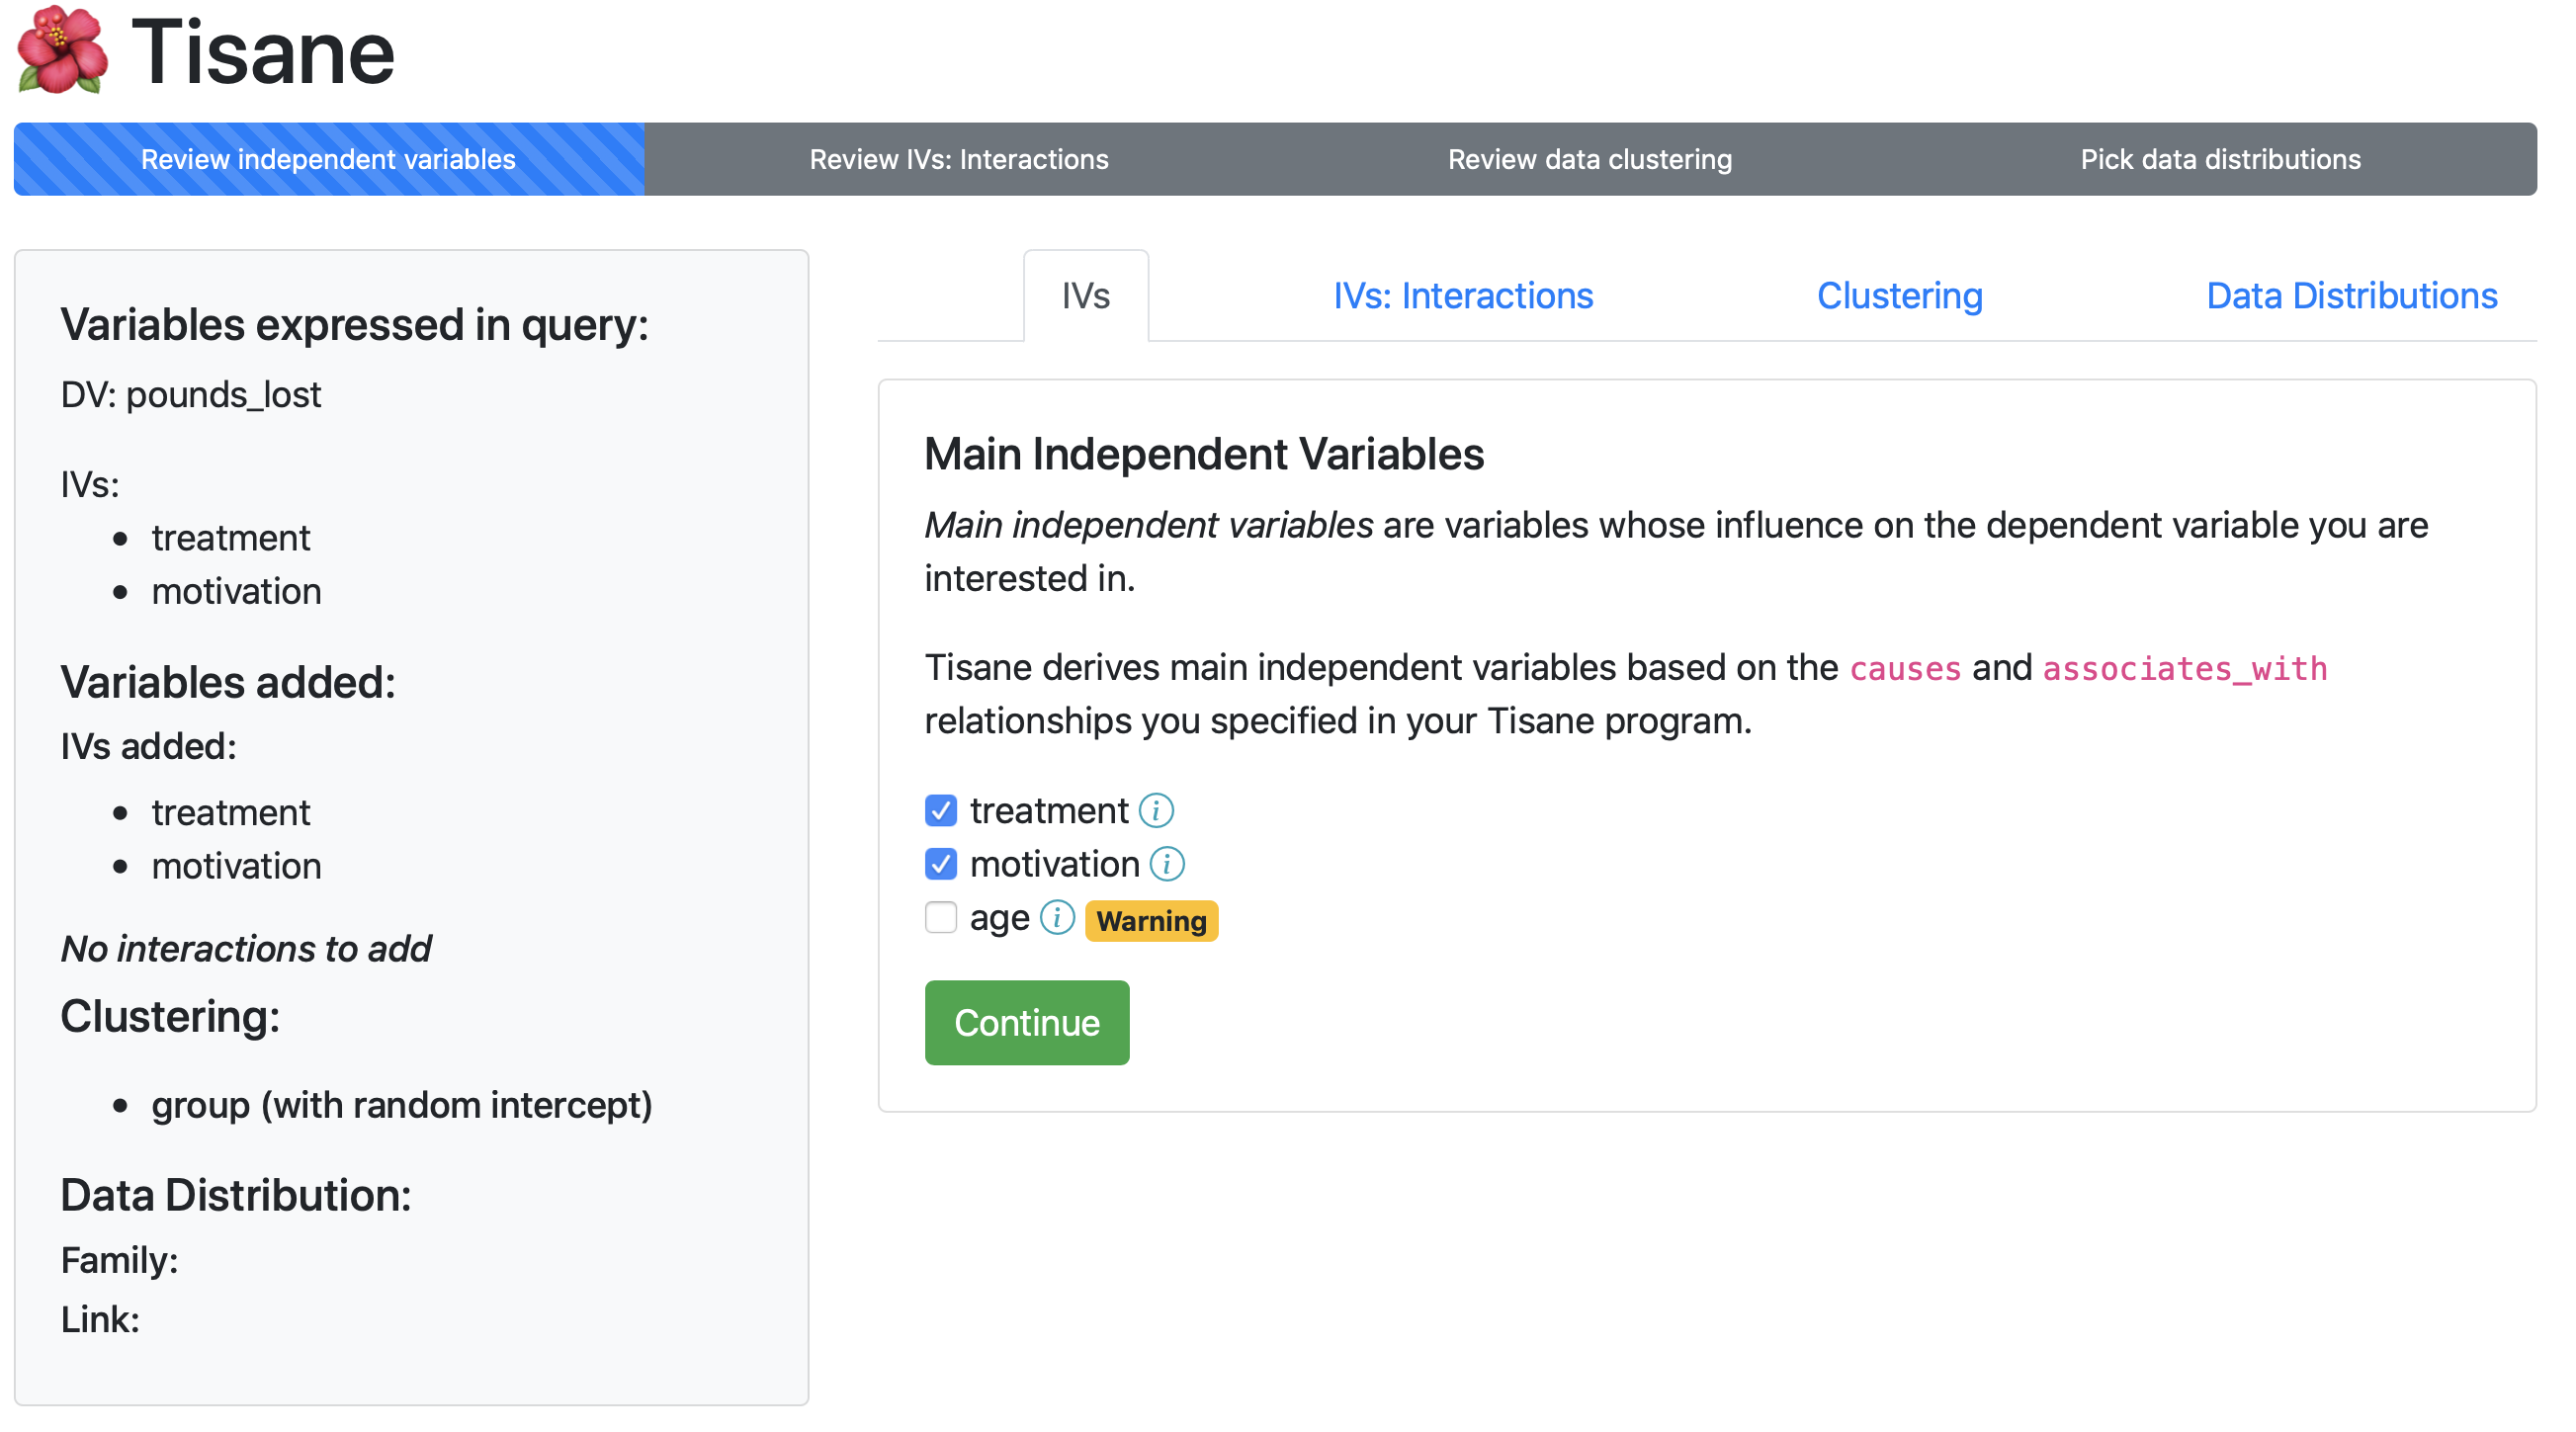
\includegraphics[width=.2\textwidth]{tisane/figures/tisane_screenshots/main_no_tooltip}};
%                % \node[below=.2cm of disambig,caption]    (disambigcaption) {\textit{Disambiguation}};
%                \node[right=of disambig,stage,text width=.2\textwidth,align=center] (code) {{\footnotesize \myequation}\\%
%                    \begin{tikzpicture}[every node/.style={rounded corners=0pt},rounded corners=0pt]
%                        \begin{axis}[rounded corners=0pt,
%                                     scatter/use mapped color={
%                                        fill=blue!80,
%                                        draw=blue!80
%                                     },
%                                     axis background/.style={fill=white},
%                                     xmin=-6.9,
%                                     xmax=6.9]
%                             \draw[gray,very thin] (axis cs:-5,-0.5) -- (axis cs:-5,0.5);
%                             \draw[gray,very thin] (axis cs:0,-0.5) -- (axis cs:0,0.5);
%                             \draw[gray,very thin] (axis cs:5,-0.5) -- (axis cs:5,0.5);
%                            \addplot[black,domain=-7:7] {0};
%                            \addplot[scatter,only marks,mark size=1.1pt] table[x=x,y=y,col sep=comma] {\loadedtable};
%                        \end{axis}
%                        \pgfresetboundingbox
%                        \path
%                                ($(current axis.south west)-(0.2cm,0.35cm)$) rectangle ($(current axis.north east)+(0,0.2cm)$);
%                    \end{tikzpicture}
%                };
%                \node   (codecaption) at ($(code.south)-(0,0.3cm)$)     {\textit{Output Code}};
%                \coordinate (ref) at ($(codecaption) + (0.5cm,0)$) {};
%                \node[caption]  (graphircaption1) at ($(codecaption)!(graphir)!(ref)$) {\textit{Graph IR}};
%                \node[caption]  (disambigcaption1) at ($(codecaption)!(disambig)!(ref)$) {\textit{Disambiguation}};
%                \node[caption]  (inputcaption)     at ($(codecaption)!(input)!(ref)$) {\textit{Input Study Design Specification}};
%                \graph{
%                    (input) ->[thick] (graphir) ->[thick] (disambig) ->[thick] (code);
%                };
%                \node at ($(current bounding box.south) + (0,-.4)$) {Interactive Compilation};
%                \node[color=white,inner sep=0pt] at ($(current bounding box.north) + (0,5pt)$) {};
%                \node[color=white,inner sep=0pt] (spacer) at ($(code.east)+(5pt,0)$) {};
%            \end{scope}
%
%            \begin{pgfonlayer}{background}
%                \node[rounded corners=4pt, draw=gray!50, fit=(bb)] {};
%                % \node[fill=gray!10, draw=none, fit=(bb)] {};
%            \end{pgfonlayer}
%            % \draw[fill=gray!30, draw=none] (current bounding box.north east) rectangle (current bounding box.south west);
%        \end{tikzpicture}
        \caption{\textbf{Overview of the Tisane system.} Analysts specify a set of variable relationships (\textit{Input Study Design Specification}). Tisane represents these in an internal graph (\textit{Graph IR}). To infer a statistical model, Tisane engages analysts in an interactive compilation process that elicits additional input from analysts in a disambiguation process (\textit{Disambiguation}) and outputs a script for fitting a valid GLM and visualizing its residuals (\textit{Output Code}).}
        \label{fig:figureSystemOverview}
        \Description{Four boxes (which we will refer to as A, B, C, and D) are shown in a row. Box A is labeled “Input Study Design Specification” and shows a text editor window where the text “import tisane as ts” is written (this is the canonical way of importing Tisane in Python, like “import pandas as pd”). Box A has an arrow pointing to Box B, which is labeled “Graph IR,” where “IR” stands for “intermediate representation.” Box B contains a directed graph with three nodes, arranged like the vertices of an isosceles triangle. The top node has a dotted arrow pointing toward the bottom left node and a solid arrow pointing at the bottom right node. The bottom right node has a dashed edge pointing toward the bottom left node and a solid edge pointing to the top node. The bottom left node has no outgoing edges. This is meant to be a icon for the Graph IR. Box B has an arrow pointing to Box C, which is labeled as “Disambiguation.” Box C contains a screenshot of the Tisane GUI. The top of the GUI has the word “Tisane” and a progress bar, which is a quarter blue and three quarters gray. A left side panel gives an overview of the current model, and shows variables expressed by the query (the dependent variable, pounds_lost, and the independent variables, treatment and motivation), the variables added (the query independent variables are listed underneath, while noting that there are no interactions to add), clustering variables (group, a random intercept), and that for data distributions, no family or link functions have been selected. Box C has an arrow pointing to Box D, which is labeled “Output Code”. The box contains an equation, Y = beta_0 + beta_1 X_1 + … + beta_n X_n, and below the equation is a plot of residuals vs. fitted values. This is meant to represent the output script that Tisane creates.}
    \end{figure*}
}

\newcommand{\figureGraphIRExample}{
    \begin{figure}[h]
\centering
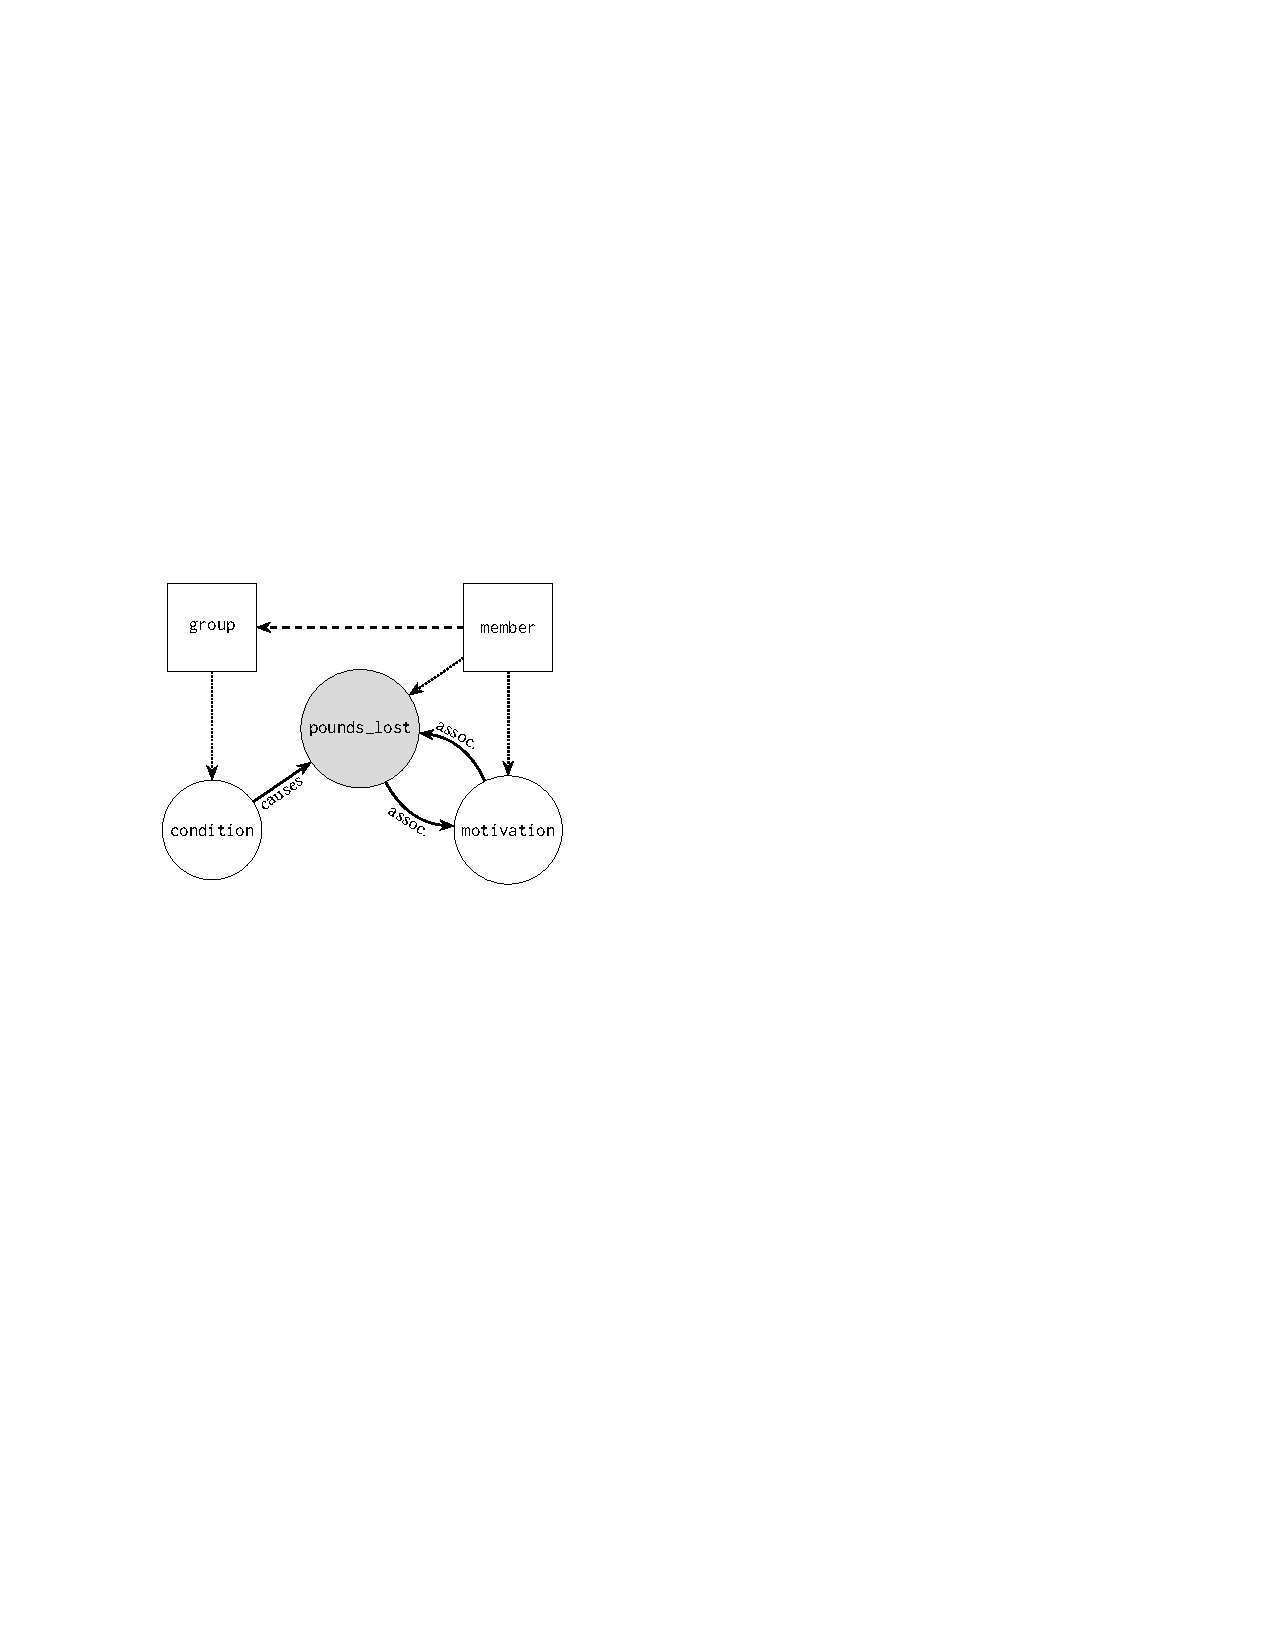
\includegraphics{tisane/figures/figure4}
%        \begin{tikzpicture}[>=Stealth,
%                            causes/.style={thick,draw=black, "causes", text=black},
%                            associates/.style={thick,draw=black, "assoc."},
%                            min/.style={minimum size=1.5cm},
%                            unit/.style={min,draw=black},
%                            measure/.style={min,circle,draw=black},
%                            has/.style={densely dotted,thick},
%                            nests/.style={dashed,thick},
%                            depvar/.style={fill=gray!30},
%                            every edge quotes/.style={fill=none,fill opacity=.9,text opacity=1,rounded corners=3pt,inner sep=2pt},
%                            tightly/.style={inner sep=1pt},
%                            loosely/.style={inner sep=.7em}]
%            \node[unit]		(group) at (0,0)			{\texttt{group}};
%            \node[unit,right=3.5cm of group]	(member)		{\texttt{member}};
%            \node[measure,below=1.75cm of member]		(motivation)	{\texttt{motivation}};
%            \coordinate (ref1) at ($(motivation.center) + (1cm, 0)$) {};
%            \node[measure] at ($(ref1)!(group.center)!(motivation.center)$)		(condition)		{\texttt{condition}};
%
%
%            \coordinate (midcoord1) at ($(group.center)!0.5!(member.center)$) {};
%            \coordinate (midcoord2) at ($(member.center)!0.5!(motivation.center)$) {};
%            \coordinate (ref) at ($(midcoord2) + (1cm, 0)$) {};
%            \node[measure,depvar] at ($(midcoord2)!(midcoord1)!(ref)$)		(poundslost)	{\texttt{pounds\_lost}};
%            % \node[measure,above right=of motivation]		(age)			{\texttt{age}};
%
%            \graph
%        %			[edge quotes={fill=white,fill opacity=.5,text opacity=1,rounded corners=4pt,inner sep=2pt}]
%                {
%                (condition) ->[causes,sloped,below,pos=0.4,loosely] (poundslost);
%                (motivation) ->[associates,bend right,pos=0.6,sloped,above] (poundslost);
%                (poundslost)	->[associates,bend right,below,sloped]	(motivation);
%                % (age)			->[associates,bend right,pos=0.3,above,sloped]	(motivation);
%                % (motivation)	->[associates,bend right,below,sloped]	(age);
%                % (age)			->[associates,bend right,pos=0.25,below,loosely,sloped]	(poundslost);
%                % (poundslost)	->[associates, bend right,very near start,sloped,below]	(age);
%                (member)		->[nests]		(group);
%                (member)		->[has]			(poundslost);
%                (member)		->[has]			(motivation);
%                % (member)		->[has]			(age);
%                (group)			->[has]			(condition);
%            };
%        \end{tikzpicture}
        \caption{The graph representation of the variables and relationships from the usage scenario. \texttt{causes} edges are labeled with ``causes''. \texttt{associates\_with} edges are labeled with ``assoc.'' Dashed edges indicate \texttt{nests\_within} relationships, and dotted edges indicate \texttt{has} relationships.}
        \label{fig:figureGraphIRExample}
        \Description{A directed graph of five nodes is depicted. The nodes are labeled “group”, “condition”, “pounds_lost”, “motivation”, and “member”, all in monospace font. The “group” node is square-shaped (indicating the node represents a Unit), and has a dotted edge pointing to the circle-shaped (indicating it’s a Measure) “condition” node. The “condition” node has a solid edge labeled “causes” pointing to the circle-shaped, gray “pounds_lost” node. The gray color indicates that “pounds_lost” was the dependent variable. The “pounds_lost” node has one outgoing solid edge labeled “assoc.” (for associative relationships), to the circle-shaped node “motivation.” The “motivation” node has an outgoing, solid “assoc.” edges to the “pounds_lost” node. The final node, “member,” is square-shaped and has a dashed outgoing edge to the “group” node and dotted outgoing edges to the “pounds_lost” and “motivation” nodes. The dashed edge means “member” nests in “group” and the dotted edges mean that “pounds_lost” and “motivation” are measures of the “member” unit.}
    \end{figure}
}

%\newcommand\betweendistance[1]{1.5cm of #1}
\newcommand{\figureCandidateMainEffects}{
%     \begin{figure*}%[h]
% \centering
% 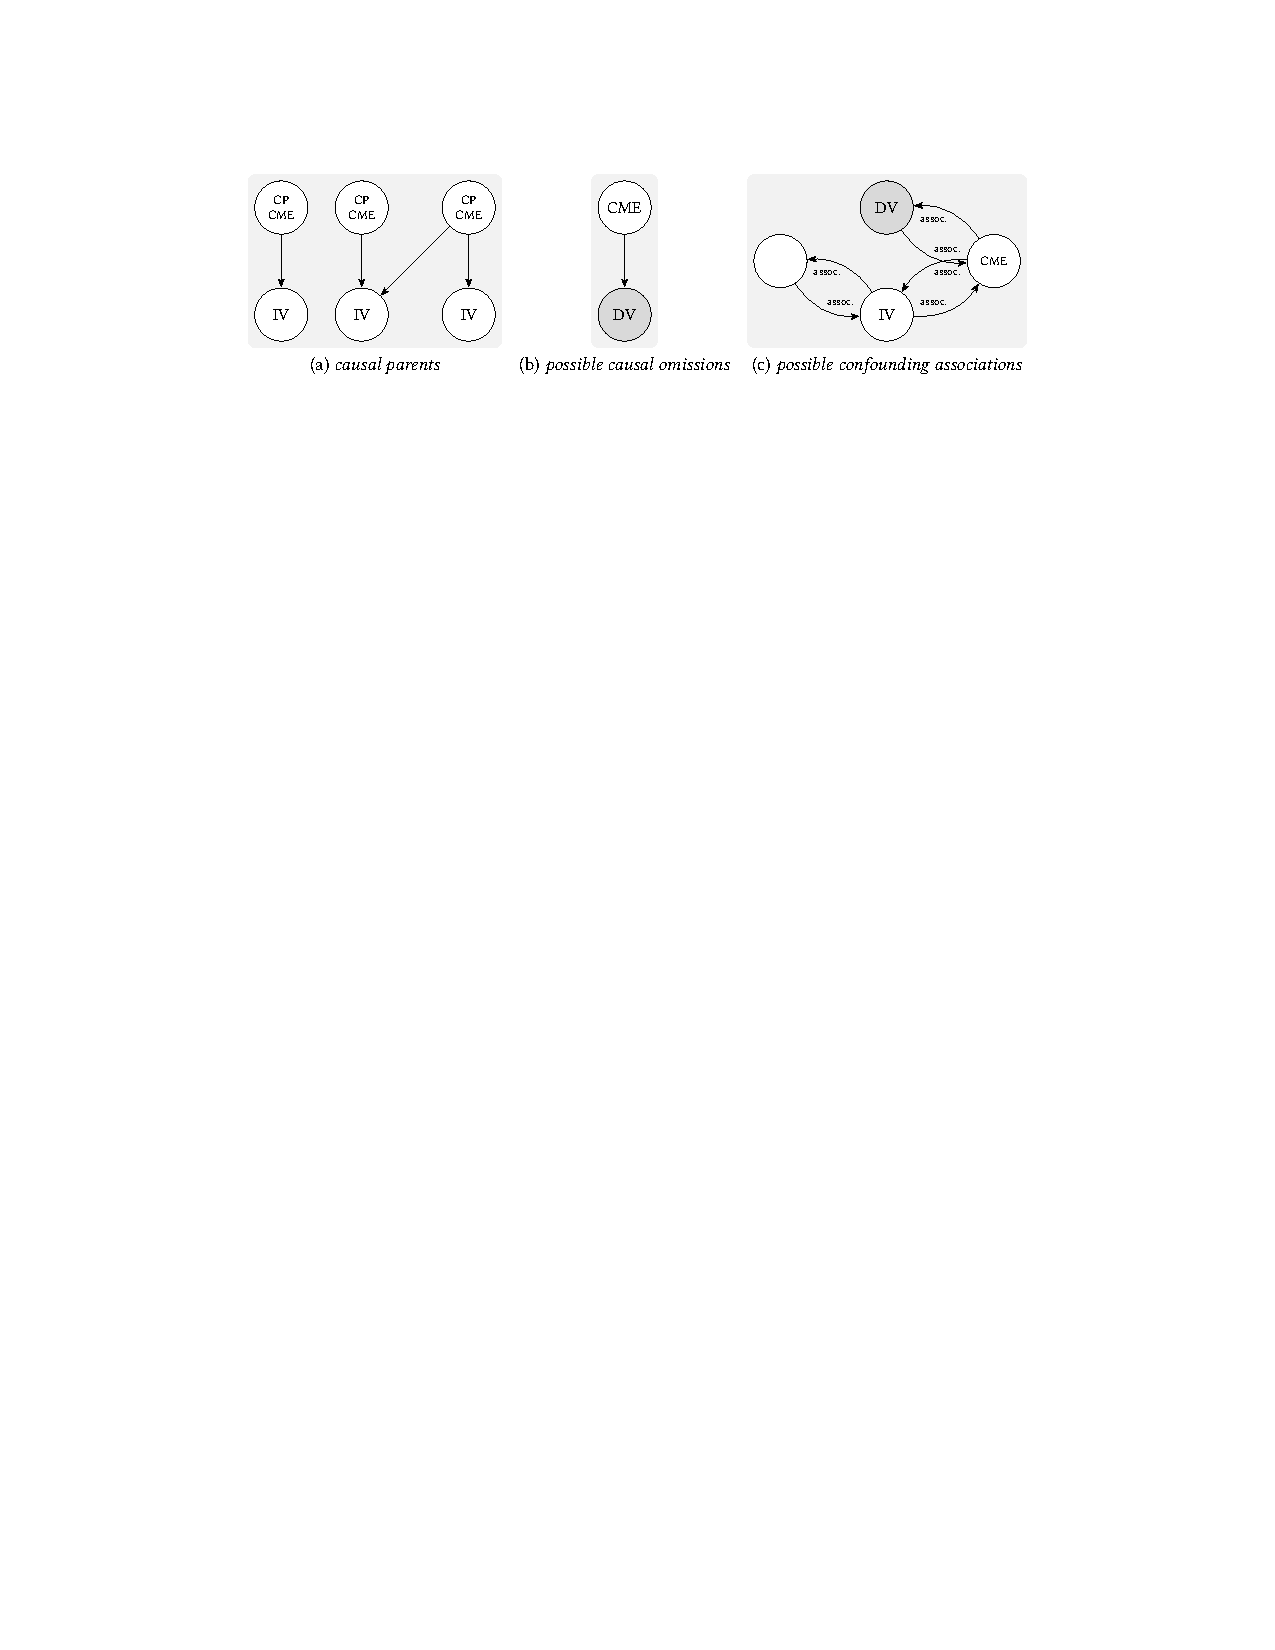
\includegraphics{tisane/figures/figure5}
       \def\arrowend{.4}
       \def\dotsbegin{.43}
       \def\dotsend{.55}
       \def\arrowbegin{.59}

       \begin{tikzpicture}
           \node[fill=gray!10,rounded corners=4pt]		(n1)			{%
               \begin{tikzpicture}[>=Stealth,
                               causes/.style={thick,draw=black, "causes",text=black},
                               associates/.style={thick,draw=black, "assoc."},
                               min/.style={minimum size=1cm},
                               unit/.style={min,draw=black},
                               measure/.style={fill=white,min,circle,draw=black},
                               has/.style={densely dotted,thick},
                               nests/.style={dashed,thick},
                               depvar/.style={fill=gray!30},
                               every edge quotes/.style={fill=none,fill opacity=.9,text opacity=1,rounded corners=3pt,inner sep=2pt},
                               tightly/.style={inner sep=1pt},
                               loosely/.style={inner sep=.7em},
                               scale=0.9,transform shape,
                               cme/.style={inner sep=0pt,text width=0.5cm,align=center,node font=\footnotesize}]
               \node[measure]	(iv1)		{IV};
               \node[measure,right=of iv1]	(iv2)		{IV};
               \node[measure,left=0.5cm of iv1]	(iv3)		{IV};
               \node[measure,above=of iv1,cme]	(p1)		{CP\\CME};
               \node[measure,above=of iv2,cme] (p2)		{CP\\CME};
               \node[measure,above=of iv3,cme]	(p3)		{CP\\CME};
               \coordinate	(point1) at ($ (p1) !.5! (p2) $)	{};
               \coordinate	(point2) at ($ (iv2) !.5! (iv3) $)	{};
               % \node[measure] (a1)	at ($ (point1) + (0,2cm) $)	{CME};
               % \draw (a1) edge[left,->] ($(a1)!\arrowend!(p1)$);
               % \draw ($(a1)!\dotsbegin!(p1)$) edge[dotted,thick]	($(a1)!\dotsend!(p1)$);
               %  edge[->] (p1);
               % \draw ($(a1)!\arrowbegin!(p1)$) edge[left,->] (p1);

               % \draw (a1) edge[right,->] ($(a1)!\arrowend!(p2)$);
               % \draw ($(a1)!\dotsbegin!(p2)$) edge[dotted,thick]	($(a1)!\dotsend!(p2)$);
               %  edge[->] (p1);
               % \draw ($(a1)!\arrowbegin!(p2)$) edge[right,->] (p2);
               \graph{
                   (p1) -> (iv1);
                   (p2) -> (iv1);
                   (p2) -> (iv2);
                   (p3) -> (iv3);
               };
           \end{tikzpicture}%
           };

           \node[right=1.5cm of n1,fill=gray!10,rounded corners=4pt]	(n2)	{%
               \begin{tikzpicture}[>=Stealth,
                                   causes/.style={thick,draw=black, "causes",text=black},
                                   associates/.style={thick,draw=black, "assoc."},
                                   min/.style={minimum size=1cm},
                                   unit/.style={min,draw=black},
                                   measure/.style={fill=white,min,circle,draw=black},
                                   has/.style={densely dotted,thick},
                                   nests/.style={dashed,thick},
                                   depvar/.style={fill=gray!30},
                                   every edge quotes/.style={fill=none,fill opacity=.9,text opacity=1,rounded corners=3pt,inner sep=2pt},
                                   tightly/.style={inner sep=1pt},
                                   loosely/.style={inner sep=.7em},
                                   scale=0.9,transform shape,
                                   cme/.style={inner sep=0pt,text width=0.5cm,align=center,node font=\footnotesize}]
                   \node[measure]  (cme)   {CME};
                   \node[measure,depvar,below=of cme]  (dv)    {DV};
                   \graph{
                       (cme) -> (dv);
                   };
               \end{tikzpicture}
           };
           \node[right=1.5cm of n2,fill=gray!10,rounded corners=4pt]	(n3)	{%
               \begin{tikzpicture}[>=Stealth,
                                   causes/.style={draw=black, "causes",text=black},
                                   associates/.style={draw=black, "assoc.",bend right},
                                   min/.style={minimum size=1cm},
                                   unit/.style={min,draw=black},
                                   measure/.style={fill=white,min,circle,draw=black},
                                   has/.style={densely dotted,thick},
                                   nests/.style={dashed,thick},
                                   depvar/.style={fill=gray!30},
                                   every edge quotes/.style={fill=none,fill opacity=.9,text opacity=1,rounded corners=3pt,inner sep=2pt,node font=\scriptsize},
                                   tightly/.style={inner sep=1pt},
                                   loosely/.style={inner sep=.7em},
                                   scale=0.9,transform shape,
                                   smalldot/.style={circle,minimum size=5pt,fill=blue,draw=none}]
                   \node[measure]	(iv)		{IV};
                   \node[measure,depvar,above=of iv]	(dv)	{DV};
                   \coordinate (center)    at ($(iv)!0.5!(dv)$);
                   \coordinate (centeroffset) at ($(center)+ (3pt,0)$);
                   \coordinate[right=of iv.east] (rightcoord);
                   \coordinate[left=of iv.west] (leftcoord);
                   \coordinate (leftleftcoord) at ($(leftcoord)-(1cm,0)$);

                   % \node[measure,left=of iv]	(m1)		{\footnotesize CME};
                   \node[measure]	(m2)	at ($(center)!(rightcoord)!(centeroffset)$)	{\footnotesize CME};
                   \node[measure]	(m3)    at ($(centeroffset)!(leftleftcoord)!(center)$)		{};

                   \graph{
                       % (iv) ->[associates,above] (m1);
                       (iv) ->[associates,above left] (m2);
                       (iv) ->[associates,below left] (m3);
                       % (m1) ->[associates,below] (iv);
                       (m2) ->[associates,below right] (iv);
                       (m3) ->[associates,above right] (iv);
                       % (m1) ->[causes,above left] (dv);
                       (m2) ->[associates,below left] (dv);
                       (dv) ->[associates,above right] (m2);
                       % (dv) ->[draw=black,"assoc.",below left,pos=0.25] (m2);
                   };
               \end{tikzpicture}%
           };
           \coordinate	(ref1)	at	($(n2.south)-(1cm,0.3cm)$) {};
           \coordinate (ref2)	at	($(n2.south)-(-1cm,0.3cm)$) {};

           \node	(cap1)	at	($(ref1)!(n1)!(ref2)$)	{(a) \textit{causal parents}};
           \node	(cap2)	at	($(ref1)!(n2)!(ref2)$)	{(b) \textit{possible causal omissions}};
           \node[inner sep=0pt]	(cap3)	at	($(ref1)!(n3)!(ref2)$)	{(c) \textit{possible confounding associations}};
           % \node[below=0.05cm of cap3,inner sep=0pt]	(cap4)	{\textit{\& possible causal omissions}};
        \end{tikzpicture}
        % \caption{Graphs demonstrating causal parents, possible causal omissions, and possible confounding associations. In graphs (a) and (b) (left and middle), all edges are causal. Independent variables are marked ``IV'', discovered candidate main effects ``CME'', dependent variables ``DV'', and causal parents ``CP''.}
        \label{fig:figureCandidateMainEffects}
    % \end{figure*}
}

\newcommand{\figureOnlyAssociatesOrCausesEdgesCandidateMainEffects}{
    \begin{figure}[H]
        \def\arrowend{.4}
        \def\dotsbegin{.43}
        \def\dotsend{.55}
        \def\arrowbegin{.59}
        \begin{tikzpicture}
            \node[fill=gray!10,rounded corners=4pt]	(n3)	{%
                \begin{tikzpicture}[>=Stealth,
                                    causes/.style={draw=black, "causes",text=black},
                                    associates/.style={draw=black, "assoc.",bend right},
                                    min/.style={minimum size=1cm},
                                    unit/.style={min,draw=black},
                                    measure/.style={fill=white,min,circle,draw=black},
                                    has/.style={densely dotted,thick},
                                    nests/.style={dashed,thick},
                                    depvar/.style={fill=gray!30},
                                    every edge quotes/.style={fill=none,fill opacity=.9,text opacity=1,rounded corners=3pt,inner sep=2pt,node font=\scriptsize},
                                    tightly/.style={inner sep=1pt},
                                    loosely/.style={inner sep=.7em},
                                    scale=0.9,transform shape]
                    \node[measure]	(iv)		{IV};
                    \node[measure,left=of iv]	(m1)		{\footnotesize CME};
                    \node[measure,right=of iv]	(m2)		{\footnotesize CME};
                    \node[measure,below=of iv]	(m3)		{};
                    \node[measure,depvar,above=of iv]	(dv)	{DV};

                    \graph{
                        % (iv) ->[associates,above] (m1);
                        (iv) ->[associates,below] (m2);
                        (iv) ->[associates,left] (m3);
                        % (m1) ->[associates,below] (iv);
                        (m2) ->[associates,above] (iv);
                        (m3) ->[associates,right] (iv);
                        (dv) ->[associates,below right] (m1);
                        (m1) ->[associates,above left] (dv);
                        % (dv) ->[draw=black,"assoc.",below right,pos=0.25] (m1);
                        % (m1) ->[associates,bend left,above left] (dv);
                        (m2) ->[associates,above right] (dv);
                        (dv) ->[draw=black,"assoc.",below left,pos=0.25] (m2);
                    };
                \end{tikzpicture}
            };

        %     \node[right=of n3,fill=gray!10,rounded corners=4pt]	(n4)	{%
        %         \begin{tikzpicture}[>=Stealth,
        %                             causes/.style={draw=black, "causes",text=black},
        %                             associates/.style={draw=black, "assoc.",bend right},
        %                             min/.style={minimum size=1cm},
        %                             unit/.style={min,draw=black},
        %                             measure/.style={fill=white,min,circle,draw=black},
        %                             has/.style={densely dotted,thick},
        %                             nests/.style={dashed,thick},
        %                             depvar/.style={fill=gray!30},
        %                             every edge quotes/.style={fill=none,fill opacity=.9,text opacity=1,rounded corners=3pt,inner sep=2pt,node font=\scriptsize},
        %                             tightly/.style={inner sep=1pt},
        %                             loosely/.style={inner sep=.7em},
        %                             scale=0.9,transform shape]
        %             % \node[measure]	(iv)		{IV};
        %             % \node[measure,left=of iv]	(m1)		{\footnotesize CME};
        %             % \node[measure,right=of iv]	(m2)		{\footnotesize CME};
        %             % \node[measure,below=of iv]	(m3)		{};
        %             \node[measure,depvar]	(dv)	{DV};
        %             \node[measure, above=of dv]     (causeleftout)  {\footnotesize CME};
        %
        %             \graph{
        %                 % (iv) ->[associates,above] (m1);
        %                 % (iv) ->[associates,below] (m2);
        %                 % (iv) ->[associates,left] (m3);
        %                 % % (m1) ->[associates,below] (iv);
        %                 % (m2) ->[associates,above] (iv);
        %                 % (m3) ->[associates,right] (iv);
        %                 % (dv) ->[associates,below right] (m1);
        %                 % (m1) ->[associates,above left] (dv);
        %                 % % (dv) ->[draw=black,"assoc.",below right,pos=0.25] (m1);
        %                 % % (m1) ->[associates,bend left,above left] (dv);
        %                 % (m2) ->[associates,above right] (dv);
        %                 % (dv) ->[draw=black,"assoc.",below left,pos=0.25] (m2);
        %             };
        %         \end{tikzpicture}
        %     };
        %     \coordinate	(ref1)	at	($(n3.south)-(1cm,0.3cm)$) {};
        %     \coordinate (ref2)	at	($(n3.south)-(-1cm,0.3cm)$) {};
        %
        %     % \node	(cap1)	at	($(ref1)!(n1)!(ref2)$)	{(a) \textit{oldest causal ancestors}};
        %     % \node	(cap2)	at	($(ref1)!(n2)!(ref2)$)	{(b) \textit{shared causal ancestors}};
        %     \node	(cap3)	at	($(ref1)!(n3)!(ref2)$)	{(a) \textit{only associative edges}};
        \end{tikzpicture}
        \caption{A graph demonstrating an edge case for candidate main effect identification, where the graph contains only associative edges. Candidate main effects are labeled ``CME'', independent variables ``IV'', and dependent variables ``DV''. Variables that are none of the above are left unlabeled. When a graph contains only associative edges, candidate main effects are identified as those that are either associated with the DV or are associated with both the IV and the DV. (Note that the graph could contain additional edges/nodes other than the ones pictured, but the additional edges would not violate any of the initial checks that Tisane makes on the graph IR.)}
        \label{fig:figureOnlyAssociatesOrCausesEdgesCandidateMainEffects}
    \end{figure}
}

\newcommand{\figureSDSLToGraphIR}{
   \def\minsize{0.8cm}
   \def\mynodefont{\normalsize}
   \def\myedgequotesfont{\scriptsize}
   \def\mynodedistance{0.9cm}
%     \begin{figure*}%[H]
% \centering
% 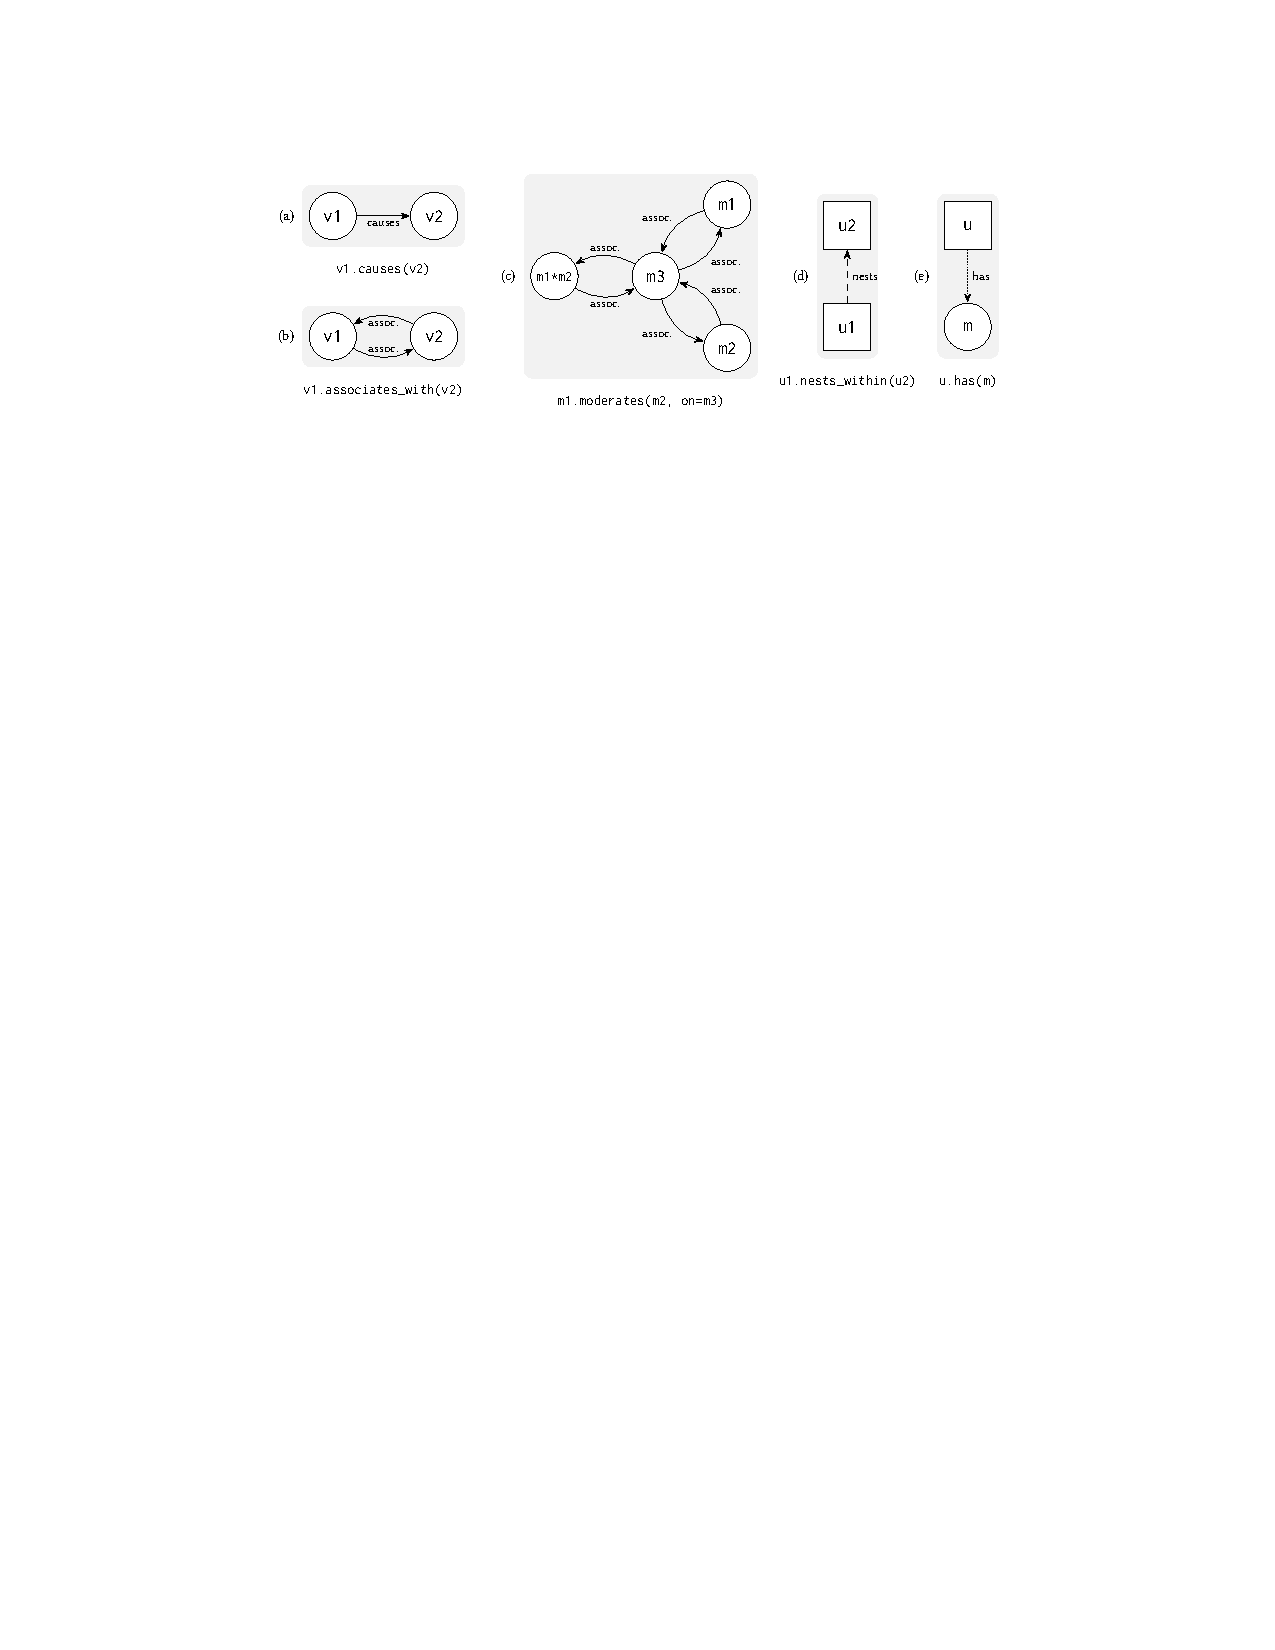
\includegraphics{tisane/figures/figure3}
       \begin{tikzpicture}[minigraph/.style={fill=gray!10,rounded corners=4pt},
                           caption/.style={node distance=.2cm,rounded corners=4pt,node font=\footnotesize},
                           closecaption/.style={node distance=.05cm,rounded corners=4pt,node font=\footnotesize}]
           \node[minigraph]		(causes)			{%
               \begin{tikzpicture}[>=Stealth,
                               every node/.style={node distance=\mynodedistance},
                               causes/.style={draw=black, "causes",text=black},
                               associates/.style={draw=black, "assoc."},
                               min/.style={minimum size=\minsize,node font=\mynodefont},
                               unit/.style={min,fill=white,draw=black},
                               measure/.style={fill=white,min,circle,draw=black},
                               has/.style={densely dotted,thick,"has"},
                               nests/.style={dashed,thick,"nests"},
                               depvar/.style={fill=gray!30},
                               every edge quotes/.style={node font=\myedgequotesfont,fill=none,fill opacity=.9,text opacity=1,rounded corners=3pt,inner sep=2pt}]
                   \node[measure]       (v1)        {\texttt{v1}};
                   \node[measure,right=of v1]  (v2) {\texttt{v2}};
                   \graph{
                       (v1) ->[causes,below] (v2);
                   };
               \end{tikzpicture}
           };

           \node[minigraph,below=of causes]		(assoc)			{%
               \begin{tikzpicture}[>=Stealth,
                               every node/.style={node distance=\mynodedistance},
                               causes/.style={draw=black, "causes",text=black},
                               associates/.style={draw=black, "assoc.",bend right},
                               min/.style={minimum size=\minsize,node font=\mynodefont},
                               unit/.style={min,fill=white,draw=black},
                               measure/.style={fill=white,min,circle,draw=black},
                               has/.style={densely dotted,thick,"has"},
                               nests/.style={dashed,thick,"nests"},
                               depvar/.style={fill=gray!30},
                               every edge quotes/.style={node font=\myedgequotesfont,fill=none,fill opacity=.9,text opacity=1,rounded corners=3pt,inner sep=2pt}]
                   \node[measure]       (v1)        {\texttt{v1}};
                   \node[measure,right=of v1]  (v2) {\texttt{v2}};
                   \graph{
                       (v1) ->[associates,above] (v2);
                       (v2) ->[associates,below] (v1);
                   };
               \end{tikzpicture}
           };
           \coordinate (mid)   at ($(causes.east)!0.5!(assoc.east)$);

           \node[minigraph,right=of mid]		(moderates)			{%
               \begin{tikzpicture}[>=Stealth,
                               every node/.style={node distance=\mynodedistance},
                               causes/.style={draw=black, "causes",text=black},
                               associates/.style={draw=black, "assoc.",bend right},
                               min/.style={minimum size=\minsize,node font=\mynodefont},
                               unit/.style={min,fill=white,draw=black},
                               measure/.style={fill=white,min,circle,draw=black},
                               has/.style={densely dotted,"has"},
                               nests/.style={dashed,thick,"nests"},
                               depvar/.style={fill=gray!30},
                               every edge quotes/.style={node font=\myedgequotesfont,fill=none,fill opacity=.9,text opacity=1,rounded corners=3pt,inner sep=2pt}]
                   \node[measure]       (v3)        {\texttt{m3}};
                   \node[measure,left=of v3,inner sep=0pt]  (v1v2) {\footnotesize \texttt{m1*m2}};
                   \node[measure,above right=of v3]    (v1)          {\texttt{m1}};
                   \node[measure,below right=of v3]    (v2)          {\texttt{m2}};
                   \coordinate (ref) at ($(v2) + (3pt,0)$);
                   % \node[unit,rounded corners=0pt] (u) at ($(v2)!(v1v2.west)!(ref)$)         {\texttt{u}};
                   \graph{
                       (v1v2) ->[associates,below] (v3);
                       (v3) ->[associates,above] (v1v2);
                       (v1) ->[associates,above left] (v3);
                       (v3) ->[associates,below right] (v1);
                       (v2) ->[associates,above right] (v3);
                       (v3) ->[associates,below left] (v2);
                       % (u)  ->[has,below,draw=gray,text=gray] (v2);
                       % (u)  ->[has,right] (v1v2);
                   };
               \end{tikzpicture}
           };

           \node[minigraph,inner sep=0pt,right=of moderates]		(nests)			{%
               \begin{tikzpicture}[>=Stealth,
                               every node/.style={node distance=\mynodedistance},
                               causes/.style={draw=black, "causes",text=black},
                               associates/.style={draw=black, "assoc.",bend right},
                               min/.style={minimum size=\minsize,node font=\mynodefont},
                               unit/.style={min,fill=white,draw=black,rounded corners=0pt},
                               measure/.style={fill=white,min,circle,draw=black},
                               has/.style={densely dotted,thick,"has"},
                               nests/.style={dashed,"nests"},
                               depvar/.style={fill=gray!30},
                               every edge quotes/.style={node font=\myedgequotesfont,fill=none,fill opacity=.9,text opacity=1,rounded corners=3pt}]
                   \node[unit]       (u1)        {\texttt{u1}};
                   \node[unit,above=of u1]  (u2) {\texttt{u2}};
                   \node[inner sep=0pt] at ($(u2.north)+(0,3pt)$)  {};
                   \node[inner sep=0pt] at ($(u2.east)+(2pt,0)$) {};
                   \node[inner sep=0pt] at ($(u2.west)-(3pt,0)$) {};
                   \node[inner sep=0pt] at ($(u1.south)-(0,3pt)$) {};
                   \coordinate (ref)   at ($(u1)!0.5!(u2)$);
                   \node[right=2pt of ref,inner sep=0pt,node font=\scriptsize] {nests};
                   \graph{
                       (u1) ->[dashed] (u2);
                   };
               \end{tikzpicture}};

           \node[minigraph,right=of nests,inner sep=0pt]		(has)			{%
               \begin{tikzpicture}[>=Stealth,
                               every node/.style={node distance=\mynodedistance},
                               causes/.style={draw=black, "causes",text=black},
                               associates/.style={draw=black, "assoc.",bend right},
                               min/.style={minimum size=\minsize,node font=\mynodefont},
                               unit/.style={min,fill=white,draw=black,rounded corners=0pt},
                               measure/.style={fill=white,min,circle,draw=black},
                               has/.style={densely dotted,"has"},
                               nests/.style={dashed,"nests"},
                               depvar/.style={fill=gray!30},
                               every edge quotes/.style={node font=\myedgequotesfont,fill=none,fill opacity=.9,text opacity=1,rounded corners=3pt,inner sep=2pt}]
                   \node[unit]       (u)        {\texttt{u}};
                   \node[measure,below=of u]  (m) {\texttt{m}};
                   \node[inner sep=0pt] at ($(u.north)+(0,3pt)$)  {};
                   \node[inner sep=0pt] at ($(u.east)+(2pt,0)$) {};
                   \node[inner sep=0pt] at ($(u.west)-(3pt,0)$) {};
                   \node[inner sep=0pt] at ($(m.south)-(0,3pt)$) {};
                   \graph{
                       (u) ->[has,right] (m);
                   };
               \end{tikzpicture}
           };

           \node[caption,below=of causes]  (causescaption) {\texttt{v1.causes(v2)}};
           \node[caption,below=of assoc]   (assoccaption)  {\texttt{v1.associates\_with(v2)}};
           \node[caption,below=of moderates]   (moderatescaption)  {\texttt{m1.moderates(m2, on=m3)}};
           \node[caption,below=of nests]       (nestscaption)      {\texttt{u1.nests\_within(u2)}};
           \node[caption,below=of has]         (hascaption)        {\texttt{u.has(m)}};
           \node[closecaption,left=of causes]   {(a)};
           \node[closecaption,left=of assoc]    {(b)};
           \node[closecaption,left=of moderates]    {(c)};
           \node[closecaption,left=of nests]    {(d)};
           \node[closecaption,left=of has]      {(e)};

       \end{tikzpicture}
        % \caption{Code snippets of conceptual and data measurement relationships written in Tisane's \SDSLlong and their representation in Tisane's graph IR. Variables are named with \texttt{u} for units, \texttt{m} for measures, and \texttt{v} for data variables that can be either units or measures. All edges depicted are those that are added due to the relationship. In the \texttt{moderates} example, we assume that \texttt{m1} and \texttt{m2} both belong to the same unit, and for simplicity, the attribution edge (labeled as ``has'') from \texttt{m1} and \texttt{m2}'s unit is not shown.}
        \label{fig:figureSDSLToGraphIR}
        % \Description{Five directed graphs are shown. All nodes are labeled with a monospaced font. The first directed graph has two nodes, labeled “v1” and “v2”, both circles. There is a solid edge from “v1” to “v2” labeled “causes”. Below this graph is a code snippet reading “v1.causes(v2)”. The second directed graph also has two nodes, also labeled “v1” and “v2” and both circles. There are solid edges from “v1” to “v2” and from “v2” to “v1”. Both edges are labeled “assoc.” Below the graph is a code snippet: “v1.associates_with(v2)”. The third directed graph contains four nodes, which are labeled “m1*m2”, “m1”, “m2”, and “m3”. All are circles. There are six edges in the graph, all solid and labeled “assoc.” The edges are from “m1*m2” to “m3”, “m3” to “m1*m2”, “m1” to “m3”, “m3” to “m1”, “m2” to “m3”, and “m3” to “m2”. Below the graph is a code snippet: “m1.moderates(m2, on=m3)”. The fourth directed graph contains two nodes, labeled “u1” and “u2”. Both are squares. There is a dashed edge labeled “nests” from “u1” to “u2”. Below the graph is the code snippet “u1.nests_within(u2)”. The fifth, and final, directed graph contains two nodes labeled “u” and “m”. “u” is square-shaped and “m” is circle-shaped. There is a dotted edge from “u” to “m”, labeled “has”. Below the graph is the code snippet “u.has(m)”.}
    % \end{figure*}
}

%\newcommand{\figureComplexModeratesGraphIR}{
%    \def\minsize{0.8cm}
%    \def\mynodefont{\normalsize}
%    \def\myedgequotesfont{\scriptsize}
%    \def\mynodedistance{0.9cm}
%    \def\myx{.5cm}
%    \def\myy{.9cm}
%    \def\mone{\texttt{m1}\xspace}
%    \def\mtwo{\texttt{m2}\xspace}
%    \def\mthree{\texttt{m3}\xspace}
%    \def\uone{\texttt{u1}\xspace}
%    \def\utwo{\texttt{u2}\xspace}
%    \def\u{\texttt{u}\xspace}
%    \def\umone{\texttt{u1*m1}\xspace}
%    \def\monetwo{\texttt{m1*m2}\xspace}
%    \begin{figure}[H]
%        \begin{tikzpicture}[minigraph/.style={fill=gray!10,rounded corners=4pt, minimum height=3.7cm},
%                            caption/.style={node distance=.2cm,rounded corners=4pt,node font=\footnotesize}]
%            \node[minigraph]		(moderates1)			{%
%                \begin{tikzpicture}[>=Stealth,
%                                every node/.style={node distance=\mynodedistance,minimum height=0cm},
%                                causes/.style={draw=black, "causes",text=black},
%                                associates/.style={draw=black, "assoc.",bend right},
%                                min/.style={minimum size=\minsize,node font=\mynodefont},
%                                unit/.style={min,fill=white,draw=black,rounded corners=0pt},
%                                measure/.style={fill=white,min,circle,draw=black},
%                                has/.style={densely dotted,"has"},
%                                nests/.style={dashed,thick,"nests"},
%                                depvar/.style={fill=gray!30},
%                                every edge quotes/.style={node font=\myedgequotesfont,fill=none,fill opacity=.9,text opacity=1,rounded corners=3pt,inner sep=2pt}]
%                    \node[measure]       (m2)        {\texttt{m2}};
%                    \node[measure,left=of m2,inner sep=0pt]  (um1) {\footnotesize \texttt{u1*m1}};
%                    \node[unit,above right=of m2]    (u1)          {\texttt{u1}};
%                    \node[measure,below right=of m2]    (m1)          {\texttt{m1}};
%                    \coordinate (ref) at ($(m1) + (3pt,0)$);
%                    \node[unit] (u2) at ($(m1)!(um1)!(ref)$)         {\texttt{u2}};
%                    \graph{
%                        (um1) ->[associates,below] (m2);
%                        (m2) ->[associates,above] (um1);
%                        (u1) ->[associates,above left] (m2);
%                        (m2) ->[associates,below right] (u1);
%                        (m1) ->[associates,above right] (m2);
%                        (m2) ->[associates,below left] (m1);
%                        (u2)  ->[has,below,draw=gray,text=gray] (m1);
%                        (u2)  ->[has,right,near start] (um1);
%                    };
%                \end{tikzpicture}
%            };
%            \node[minigraph, right=of moderates1]		(moderates2)			{%
%                \begin{tikzpicture}[>=Stealth,
%                                every node/.style={node distance=\mynodedistance,minimum height=0cm},
%                                causes/.style={draw=black, "causes",text=black},
%                                associates/.style={draw=black, "assoc.",bend right},
%                                min/.style={minimum size=\minsize,node font=\mynodefont},
%                                unit/.style={min,fill=white,draw=black,rounded corners=0pt},
%                                measure/.style={fill=white,min,circle,draw=black},
%                                has/.style={densely dotted,"has"},
%                                old/.style={draw=gray,text=gray},
%                                nests/.style={dashed,thick,"nests"},
%                                depvar/.style={fill=gray!30},
%                                every edge quotes/.style={node font=\myedgequotesfont,fill=none,fill opacity=.9,text opacity=1,rounded corners=3pt,inner sep=2pt}]
%                    \node[measure]       (v3)        {\texttt{m3}};
%                    \node[measure,left=of v3,inner sep=0pt]  (v1v2) {\footnotesize \texttt{m1*m2}};
%                    \node[measure,above right=of v3]    (v1)          {\texttt{m1}};
%                    \node[measure,below right=of v3]    (v2)          {\texttt{m2}};
%                    \coordinate (ref) at ($(v2) + (3pt,0)$);
%                    \coordinate (ref1) at ($(v1) + (3pt,0)$);
%                    \node[unit] (u) at ($(v2)!(v1v2.west)!(ref)$)         {\texttt{u2}};
%                    \node[unit] (u2) at ($(v1)!(v1v2.west)!(ref1)$)       {\texttt{u1}};
%                    \graph{
%                        (v1v2) ->[associates,below] (v3);
%                        (v3) ->[associates,above] (v1v2);
%                        (v1) ->[associates,above left] (v3);
%                        (v3) ->[associates,below right] (v1);
%                        (v2) ->[associates,above right] (v3);
%                        (v3) ->[associates,below left] (v2);
%                        (u)  ->[has,below,old] (v2);
%                        (u)  ->[has,right,near start] (v1v2);
%                        (u2) ->[has,above,old] (v1);
%                        (u2) ->[has,right,near start] (v1v2);
%                    };
%                \end{tikzpicture}
%            };
%
%            \node[minigraph, right=of moderates2]		(moderates3)			{%
%                \begin{tikzpicture}[>=Stealth,
%                                every node/.style={node distance=\mynodedistance,minimum height=0cm},
%                                causes/.style={draw=black, "causes",text=black},
%                                associates/.style={draw=black, "assoc.",bend right},
%                                min/.style={minimum size=\minsize,node font=\mynodefont},
%                                unit/.style={min,fill=white,draw=black,rounded corners=0pt},
%                                measure/.style={fill=white,min,circle,draw=black},
%                                has/.style={densely dotted,"has"},
%                                old/.style={draw=gray,text=gray},
%                                nests/.style={dashed,thick,"nests"},
%                                depvar/.style={fill=gray!30},
%                                every edge quotes/.style={node font=\myedgequotesfont,fill=none,fill opacity=.9,text opacity=1,rounded corners=3pt,inner sep=2pt}]
%                    \node[measure]       (v3)        {\texttt{m3}};
%                    \node[measure,left=2cm of v3,inner sep=0pt]  (v1v2) {\footnotesize \texttt{m1*m2}};
%                    \node[measure,above right=1.5cm and 0.6cm of v3]    (v1)          {\texttt{m1}};
%                    \node[measure,above left=0.9cm and 0.5cm of v3]    (v2)          {\texttt{m2}};
%                    \coordinate (ref) at ($(v2) + (3pt,0)$);
%                    \coordinate (ref1) at ($(v1) + (3pt,0)$);
%                    % \node[unit] (u) at ($(v2)!(v1v2.west)!(ref)$)         {\texttt{u1}};
%                    \node[unit] (u2) at ($(v1)!(v1v2.west)!(ref1)$)       {\texttt{u}};
%                    \graph{
%                        (v1v2) ->[associates,above] (v3);
%                        (v3) ->[associates,below] (v1v2);
%                        (v1) ->[associates,sloped,below] (v3);
%                        (v3) ->[associates,sloped,above] (v1);
%                        (v2) ->[associates,sloped,above] (v3);
%                        (v3) ->[associates,sloped,below] (v2);
%                        % (u)  ->[has,below,old] (v2);
%                        % (u)  ->[has,right] (v1v2);
%                        (u2) ->[has,above,old] (v1);
%                        (u2) ->[has,below left,old] (v2);
%                        (u2) ->[has,right] (v1v2);
%                    };
%                \end{tikzpicture}
%            };
%            \node[caption,below=of moderates1]      {(a) \texttt{m1.moderates(u1, on=m2)}};
%            \node[caption,below=of moderates2]      {(b) \texttt{m1.moderates(m2, on=m3)}};
%            \node[caption,below=of moderates3]      {(c) \texttt{m1.moderates(m2, on=m3)}};
%        \end{tikzpicture}
%        \caption{More complex examples of \texttt{moderates} written in Tisane's \SDSLlong, and their representation in Tisane's graph IR. Variables are named with \texttt{u} for units, \texttt{m} for measures, and \texttt{v} for data variables that can be either units or measures. Black edges have been added due to the \texttt{moderates} relationship. Gray edges already existed in the graph. In (a), only \mone is a measure, whose unit is \utwo, so \umone inherits an attribution edge only from \utwo. In (b), \mone and \mtwo are measures, with units \uone and \utwo respectively, so \monetwo inherits attribution edges from both \uone and \utwo. In (c), measures \mone and \mtwo share a unit, \u, and \monetwo inherits only one attribution edge from \u.}
%        \label{fig:figureComplexModeratesGraphIR}
%    \end{figure}
%}


%\newcommand{\tableClusteringExamples}{
%    \begin{table}
%        \caption{\textbf{Common types of data clustering that Tisane
%        automatically accounts for inferred statistical models.} \ej{Should the
%        examples come from the preliminary expressive coverage analysis?} There
%        are three types of clustering that Tisane detects based on analysts'
%        data measurement relationships. Below are examples for each type of
%        clustering and the maximal random effects~\cite{barr2013random} Tisane
%        derives. Tisane also derives random effects for interaction terms based
%        on Barr's updated
%        rules~\cite{barr2013randomUpdated}.}\label{table:clusteringExamples}
%        % \begin{tabular}{p{0.2\linewidth} | p{0.5\linewidth} | p{0.3\linewidth}}
%        \begin{tabular}{>{\raggedright}p{0.2\linewidth}>{\raggedright}p{0.5\linewidth}>{\raggedright\arraybackslash}p{0.3\linewidth}}
%            Type of clustering	&	Example	&	Random effects Tisane infers \\
%            \hline
%            Repeated measures	&	Typing speed is measured once per day for five days. 	&	Random intercept for individuals, random intercept for days \\
%            Hierarchical data 	&	Adults in exercise groups participate in a study where each group receives a different training regimen.~\cite{cohen2013applied}	&	Random intercept for group \\
%            Non-nesting composition 	&	{Participants are assigned two conditions, each representing one of the five senses. In each condition, participants use an input device that leverages a different sense. Each input device is designed for exactly one sense, so input devices are not independent of condition.}	&	Random intercept and slope for participants, random intercept for input devices
%        \end{tabular}
%        \label{tab:tableClusteringExamples}
%    \end{table}
%}
%
%\newcommand{\tableFamilyLinkFunctions}{
%  \begin{table}[h]
%    \caption{The available family and link functions in Tisane. Tisane generates code to fit models using \texttt{statsmodels} and \texttt{pymer4}. The package \texttt{statsmodels} supports GLMs without mixed-effects and a wider variety of family and link function combinations. The package \texttt{pymer4} supports GLMs with mixed effects and has much more limited support for family and link functions. As \texttt{statsmodels} and \texttt{pymer} add more support, Tisane can be extended.}
%    \begin{tabular}{lll} \hline
%    %   \multirow{3}{*}{\multicolumn{1}{c}{Family functions}}	&	\multicolumn{2}{c}{Link functions (*default)} \\ \cline{2-3}
%      &	\multicolumn{2}{c}{Link functions (*default)} \\ \cline{2-3}
%      \multicolumn{1}{c}{Family functions} & \multicolumn{1}{>{\raggedright}p{0.35\linewidth}}{Generalized linear models without mixed effects (\texttt{statsmodels})} & \multicolumn{1}{>{\raggedright}p{0.35\linewidth}}{Generalized linear models with mixed effects (\texttt{pymer4})}	\\ \hline
%      \multirow{1}{*}{Gaussian} 	&	\multicolumn{1}{>{\raggedright}p{0.35\linewidth}}{Identity*, Inverse, Log}	&	\multirow{1}{*}{Identity*}	\\
%      Inverse Gaussian	&	Identity, Inverse, Inverse Squared*, Log	&	Inverse Squared*	\\
%      Gamma	&	Identity, Inverse*, Log 	&	Inverse*	\\
%      Poisson 	&	Identity, Log*, Square Root	&	Log*	\\
%      Binomial	&	Cauchy, CLogLog, Log, Logit*, Probit,	&	Logit*	\\
%      Negative Binomial	&	Identity, Log*, Logit, Probit	&	N/A	\\
%      Tweedie Family	&	Log*, Power	& N/A		\\
%    \end{tabular}
%    \label{tab:tableFamilyLinkFunctions}
%  \end{table}
%}

\newcommand{\michaelsFirstModel}{\par\vspace*{6pt}%
{\centering
\noindent\hspace*{-10pt}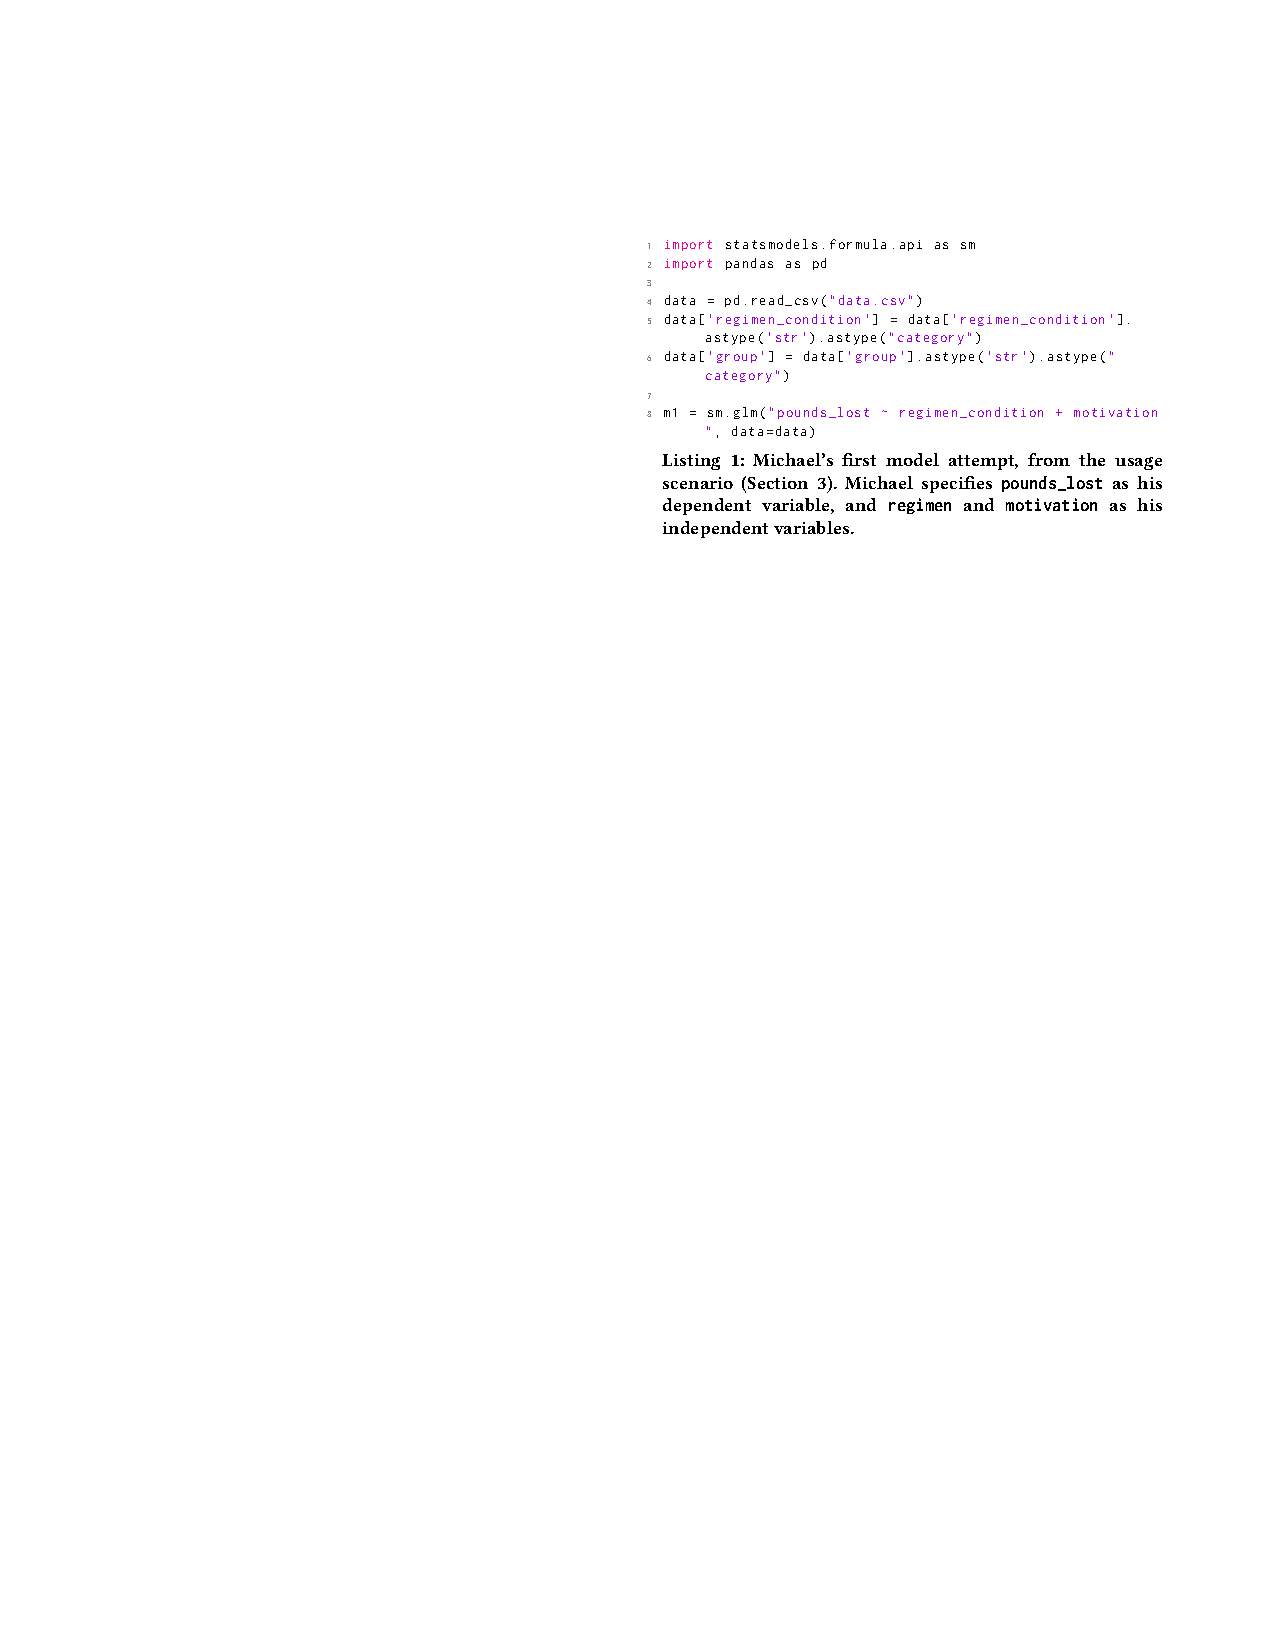
\includegraphics{tisane/figures/lst1}}
%\label={lst:michaelsFirstModel}
%    \lstinputlisting[
%        language=Python,
%        caption={Michael's first model attempt, from the usage scenario (\ref{sec:usage_scenario}). Michael specifies \poundslost as his dependent variable, and \regimen and \motivation as his independent variables.},
%        linerange={1-8},
%        label={lst:michaelsFirstModel}
%    ]{code/usage_scenario_group_exercise_statsmodels.py}
}

\newcommand{\michaelsSecondModel}{\par\vspace*{6pt}%
{\centering
\noindent\hspace*{-10pt}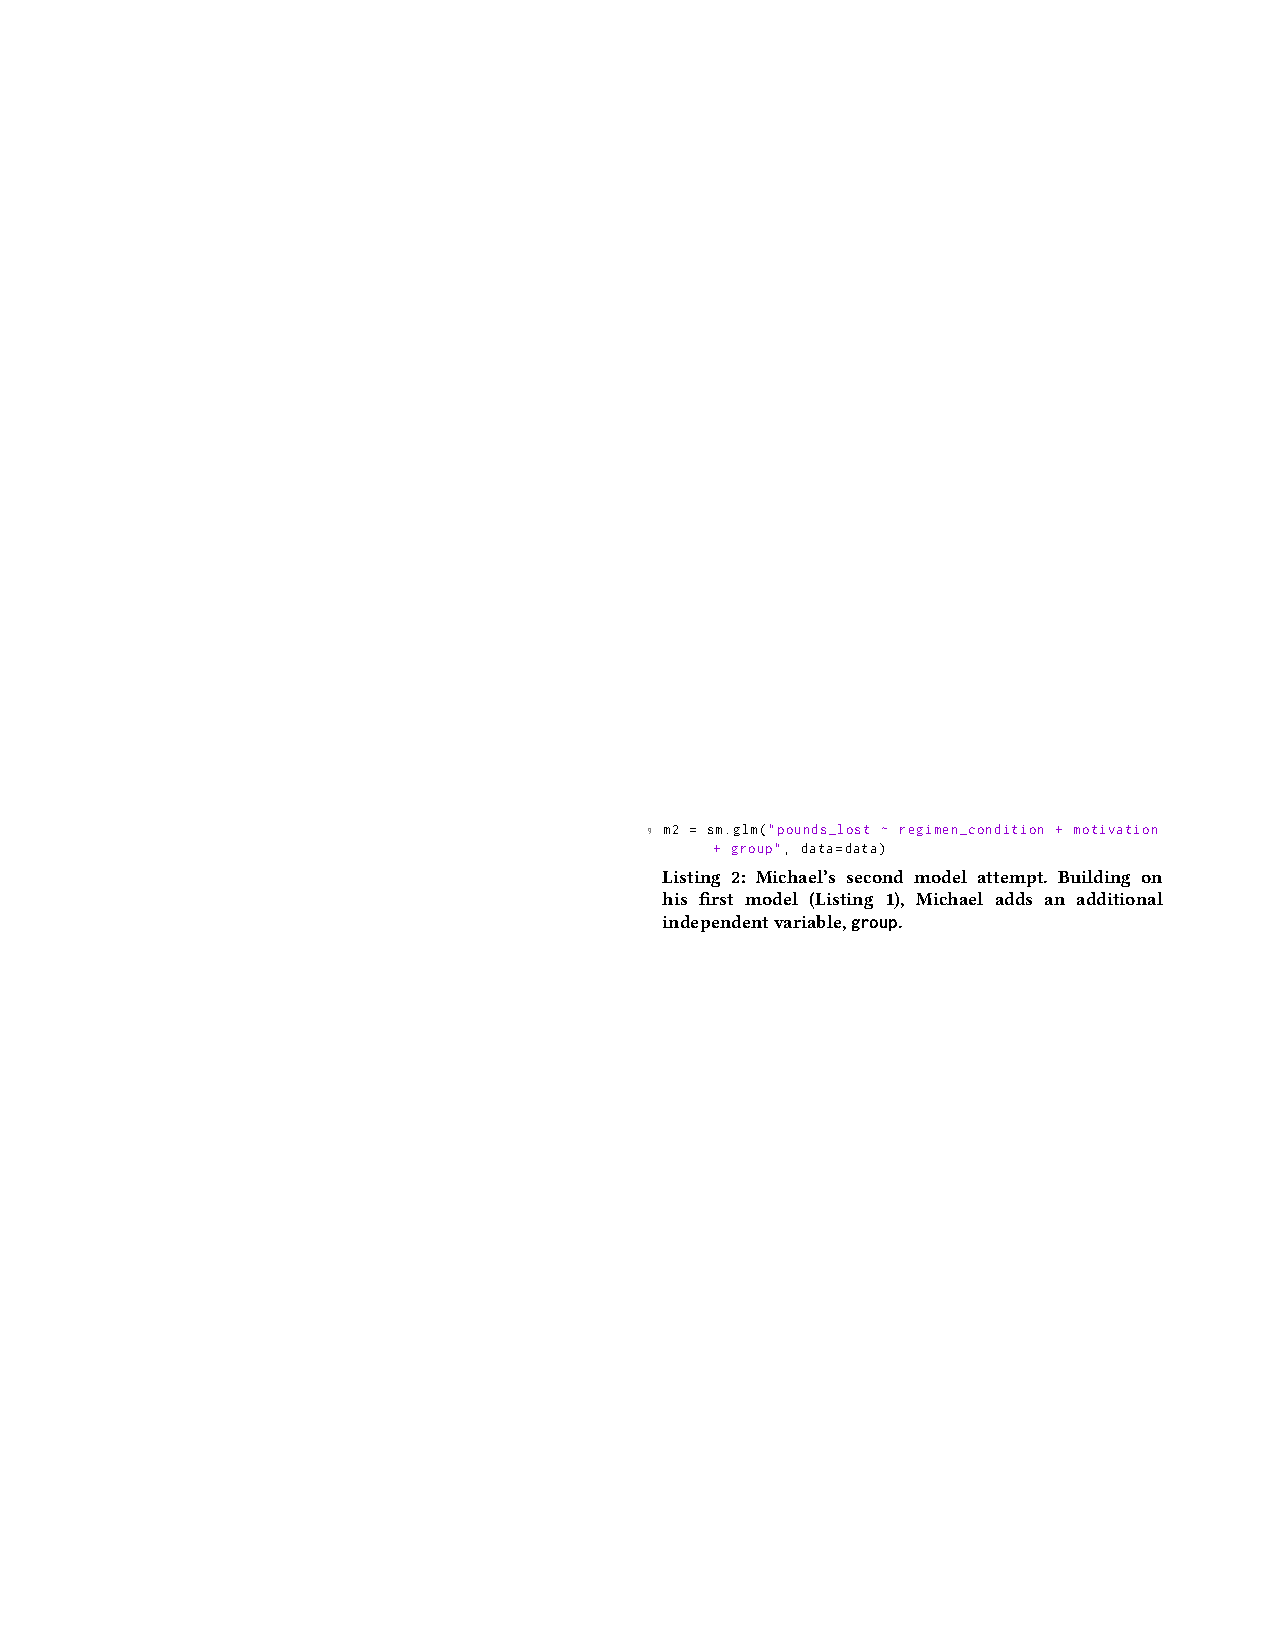
\includegraphics{tisane/figures/lst2}}
%    \lstinputlisting[
%        language=Python,
%        caption={Michael's second model attempt. Building on his first model (\ref{lst:michaelsFirstModel}), Michael adds an additional independent variable, \group.},
%        linerange={9},
%        firstnumber=9,
%        label={lst:michaelsSecondModel}
%    ]{code/usage_scenario_group_exercise_statsmodels.py}
}

\newcommand{\groupExerciseCode}{
    \lstinputlisting[language=Python, caption={Example Tisane program from usage scenario (\ref{sec:usage_scenario}).
    A Tisane program consists of a set of observed variables, expresses relationships between them, and queries Tisane for a statistical model by specifying a study design.
    Based on this input program, Tisane involves analysts in a disambiguation process to generate a final output statistical modeling script.}, label={lst:groupExerciseCode}]{code/usage_scenario_group_exercise.py}
}

\newcommand{\groupExerciseCodeVariables}{\par\vspace*{6pt}%
{\centering
\noindent\hspace*{-10pt}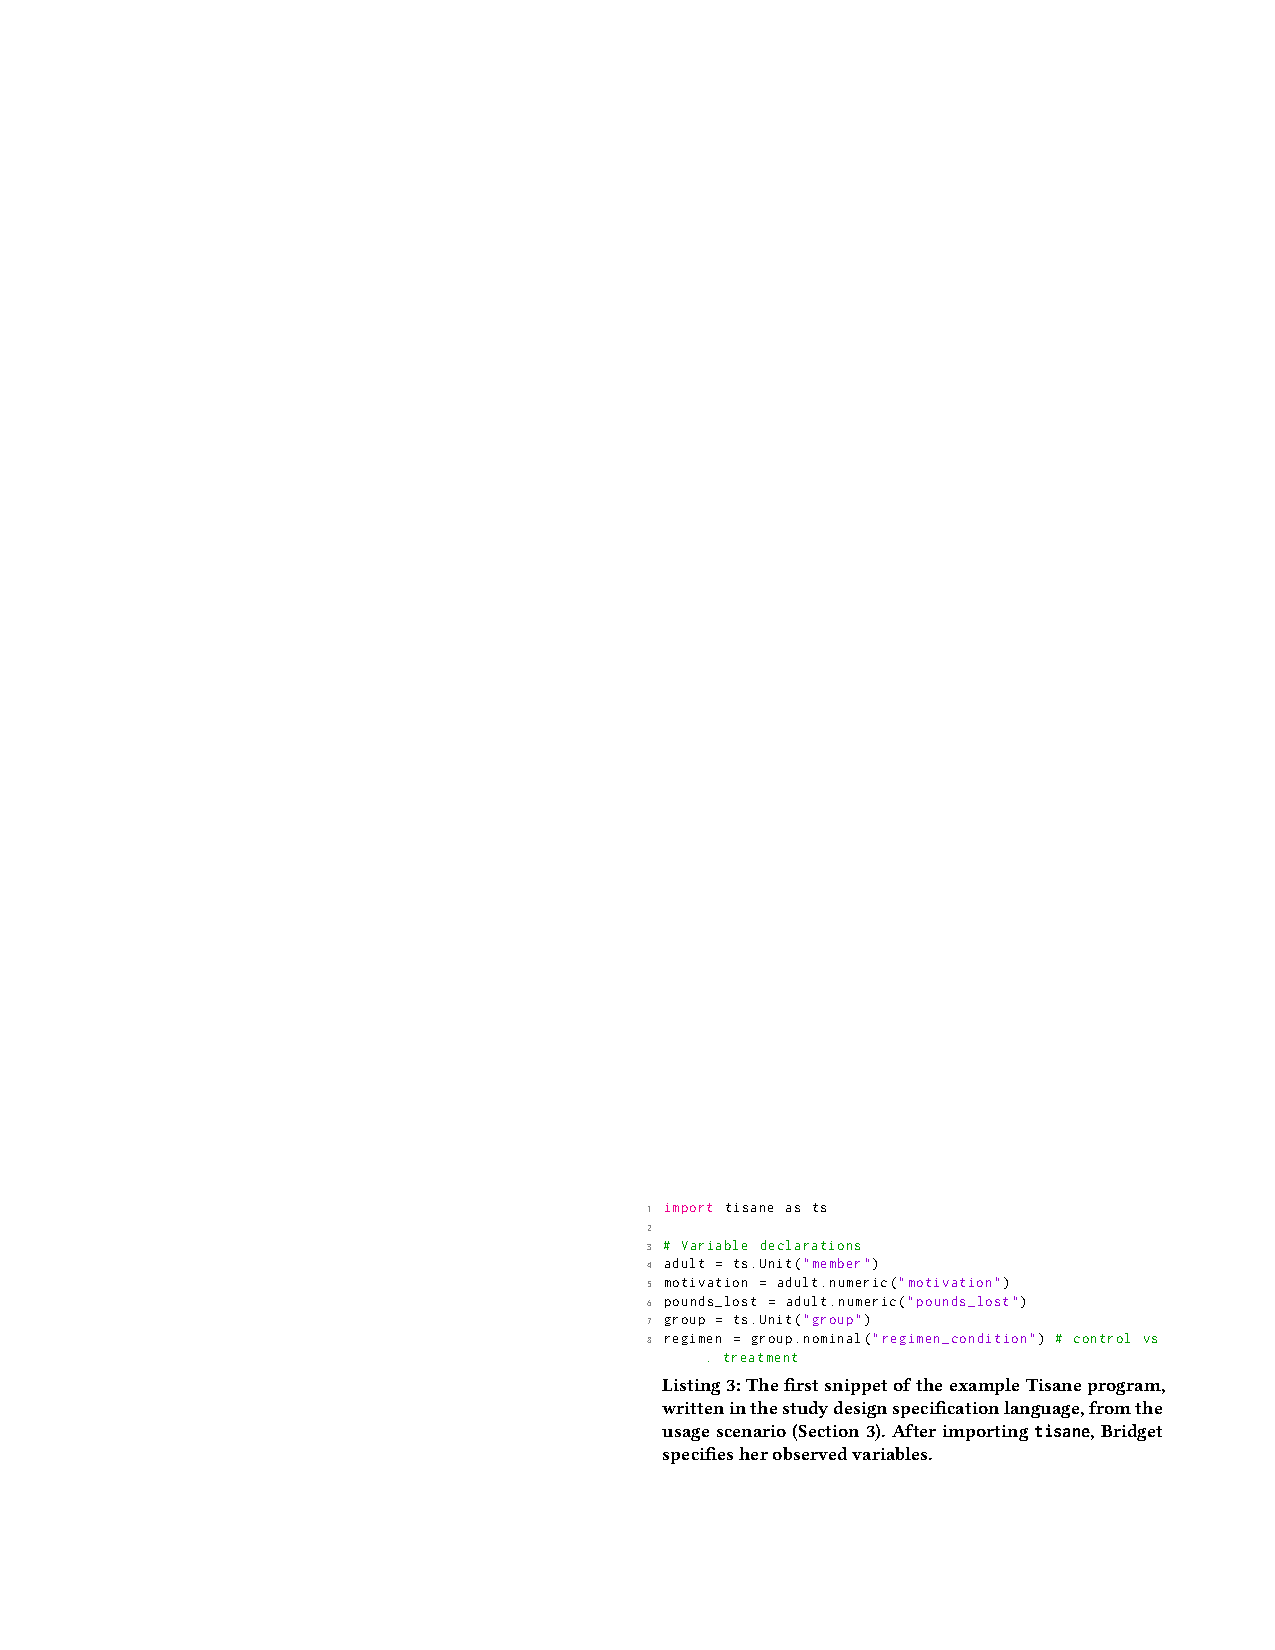
\includegraphics{tisane/figures/lst3}}
%    \lstinputlisting[language=Python,caption={The first snippet of the example Tisane program, written in the \SDSLlong, from the usage scenario (\ref{sec:usage_scenario}). After importing \texttt{tisane}, Bridget specifies her observed variables.}, linerange={1-8},label={lst:groupExerciseCodeVariables}]{code/usage_scenario_group_exercise.py}
}

\newcommand{\groupExerciseCodeRelationships}{\par\vspace*{6pt}%
{\centering
\noindent\hspace*{-10pt}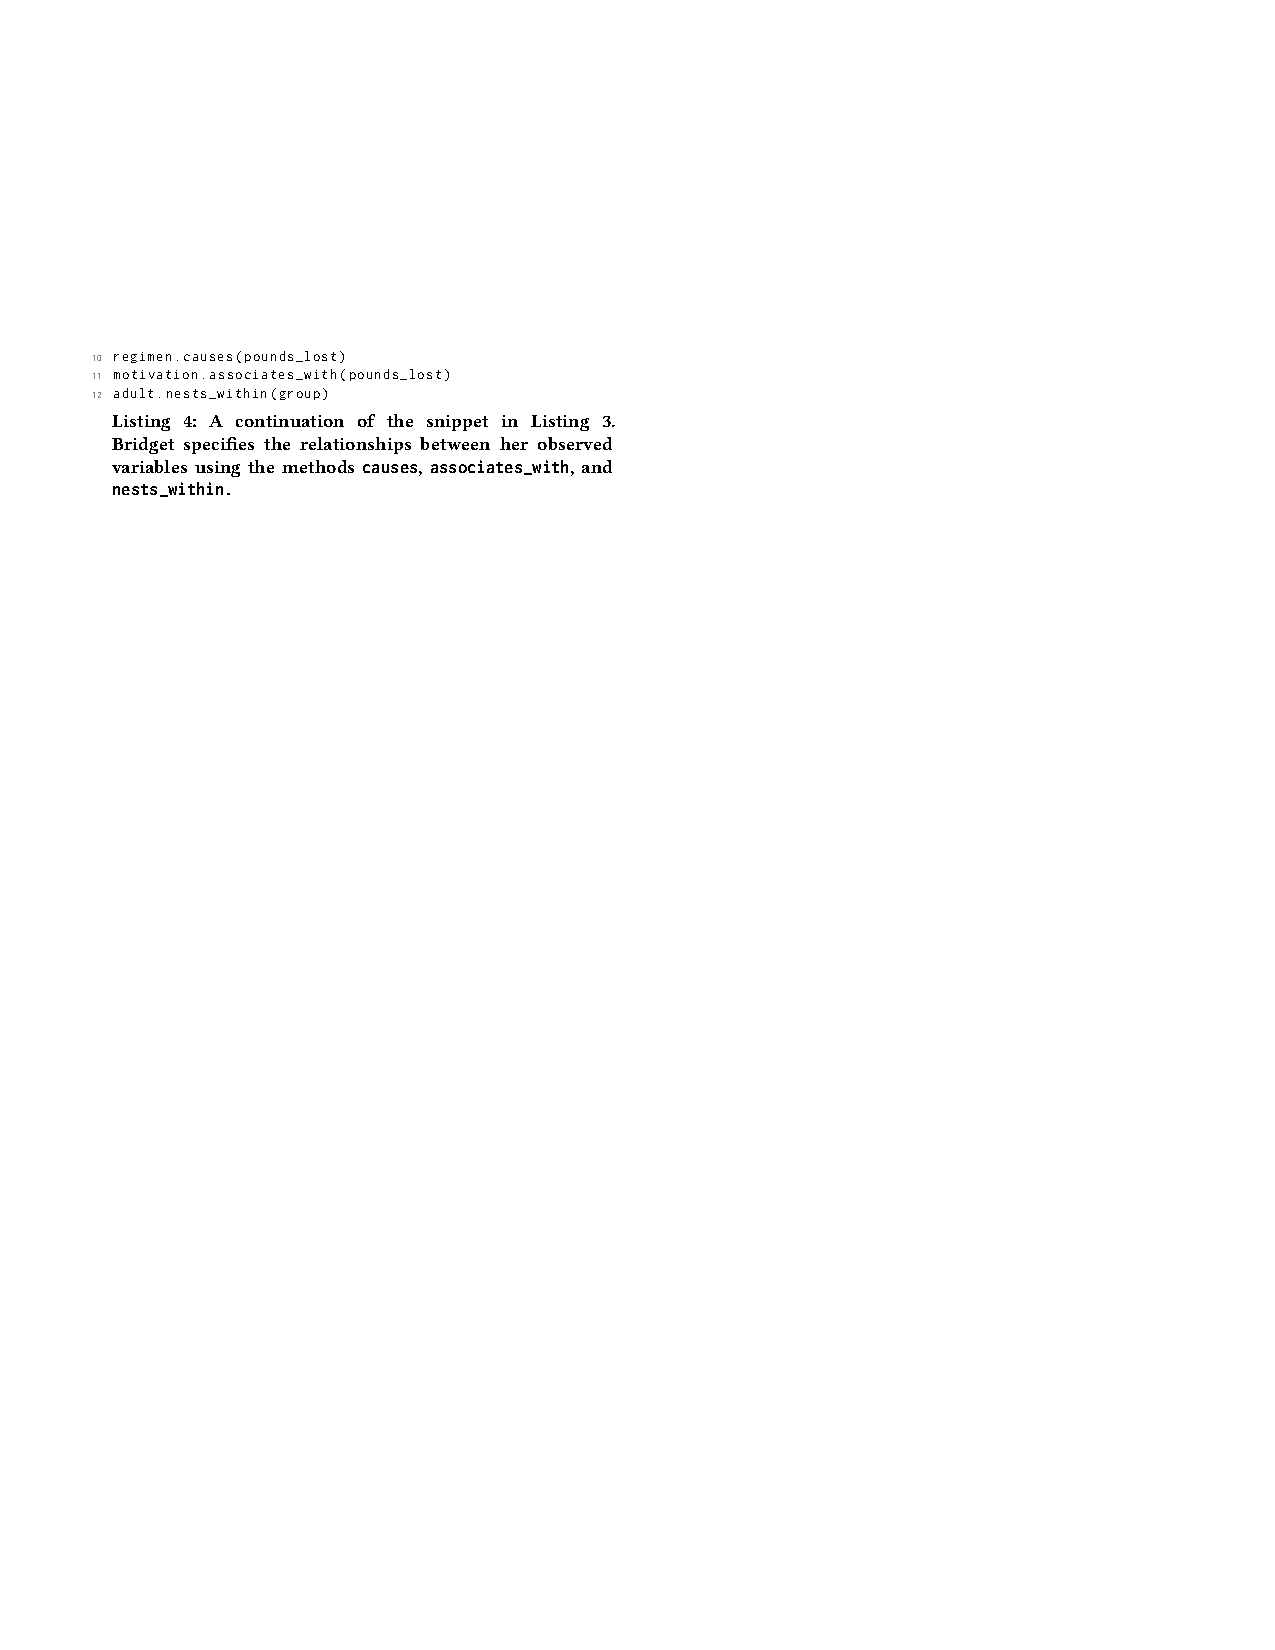
\includegraphics{tisane/figures/lst4}}
%    \lstinputlisting[language=Python,caption={A continuation of the snippet in~\ref{lst:groupExerciseCodeVariables}. Bridget specifies the relationships between her observed variables using the methods \texttt{causes}, \texttt{associates\_with}, and \texttt{nests\_within.}}, linerange={10-12},firstnumber=10,label={lst:groupExerciseCodeRelationships}]{code/usage_scenario_group_exercise.py}
}

\newcommand{\groupExerciseCodeDesignAndQuery}{\par\vspace*{6pt}%
{\centering
\noindent\hspace*{-10pt}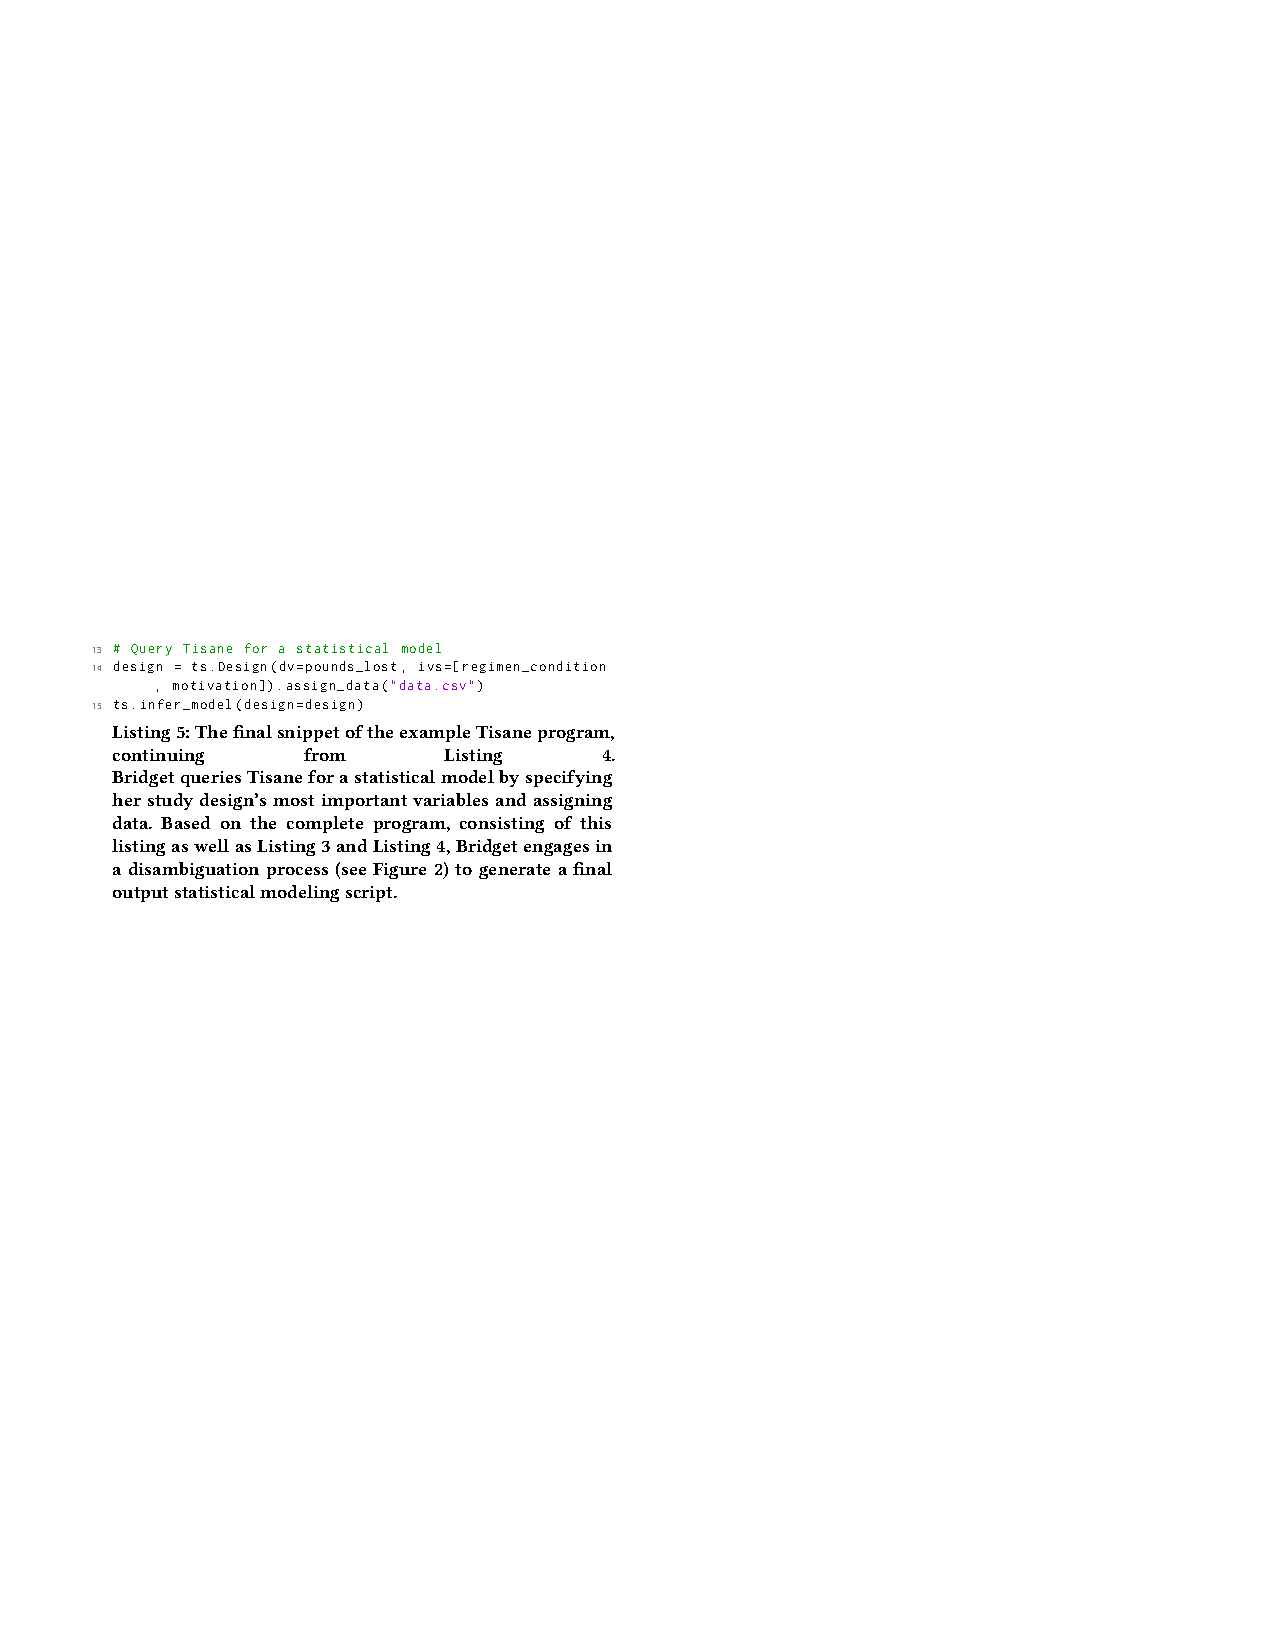
\includegraphics{tisane/figures/lst5}}
%    \lstinputlisting[language=Python,caption={The final snippet of the example Tisane program, continuing from~\ref{lst:groupExerciseCodeRelationships}. Bridget queries Tisane for a statistical model by specifying her study design's most important variables and assigning data. Based on the complete program, consisting of this listing as well as~\ref{lst:groupExerciseCodeVariables} and~\ref{lst:groupExerciseCodeRelationships}, Bridget engages in a disambiguation process (see~\ref{fig:groupExerciseDisambiguation}) to generate a final output statistical modeling script.}, linerange={13-15},firstnumber=13,label={lst:groupExerciseCodeDesignAndQuery}]{code/usage_scenario_group_exercise.py}
}

\newcommand{\groupExerciseOutputModel}{\par\vspace*{6pt}%
{\centering
\noindent\hspace*{-10pt}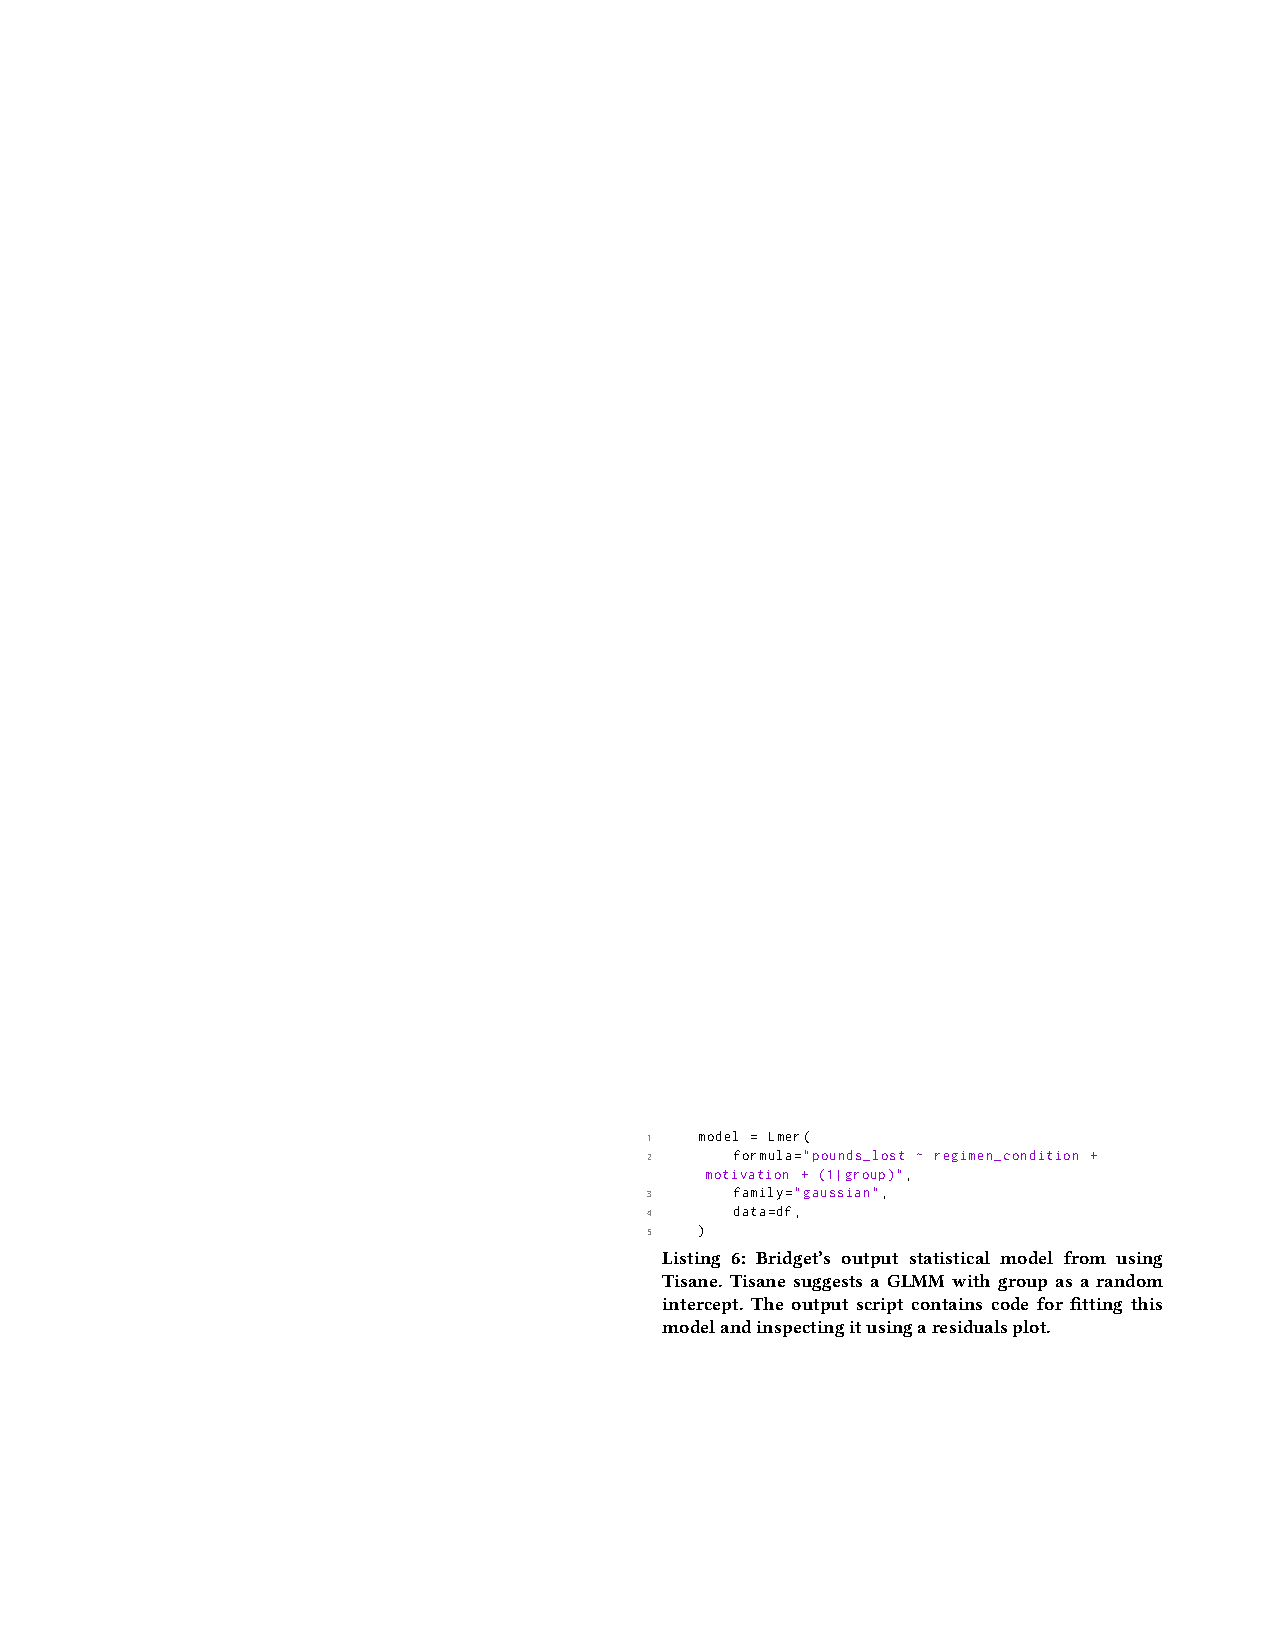
\includegraphics{tisane/figures/lst6}}
%    \lstinputlisting[
%        language=Python,
%        caption={Bridget's output statistical model from using Tisane. Tisane suggests a GLMM with group as a random intercept. The output script contains code for fitting this model and inspecting it using a residuals plot.},
%        linerange={18-22},
%        % firstnumber=18,
%        label={lst:groupExerciseOutputModel}
%    ]{code/usage_scenario_tisane_output.py}
}

\newcommand{\groupExerciseDisambiguation}{
    \begin{figure*}
        \centering
        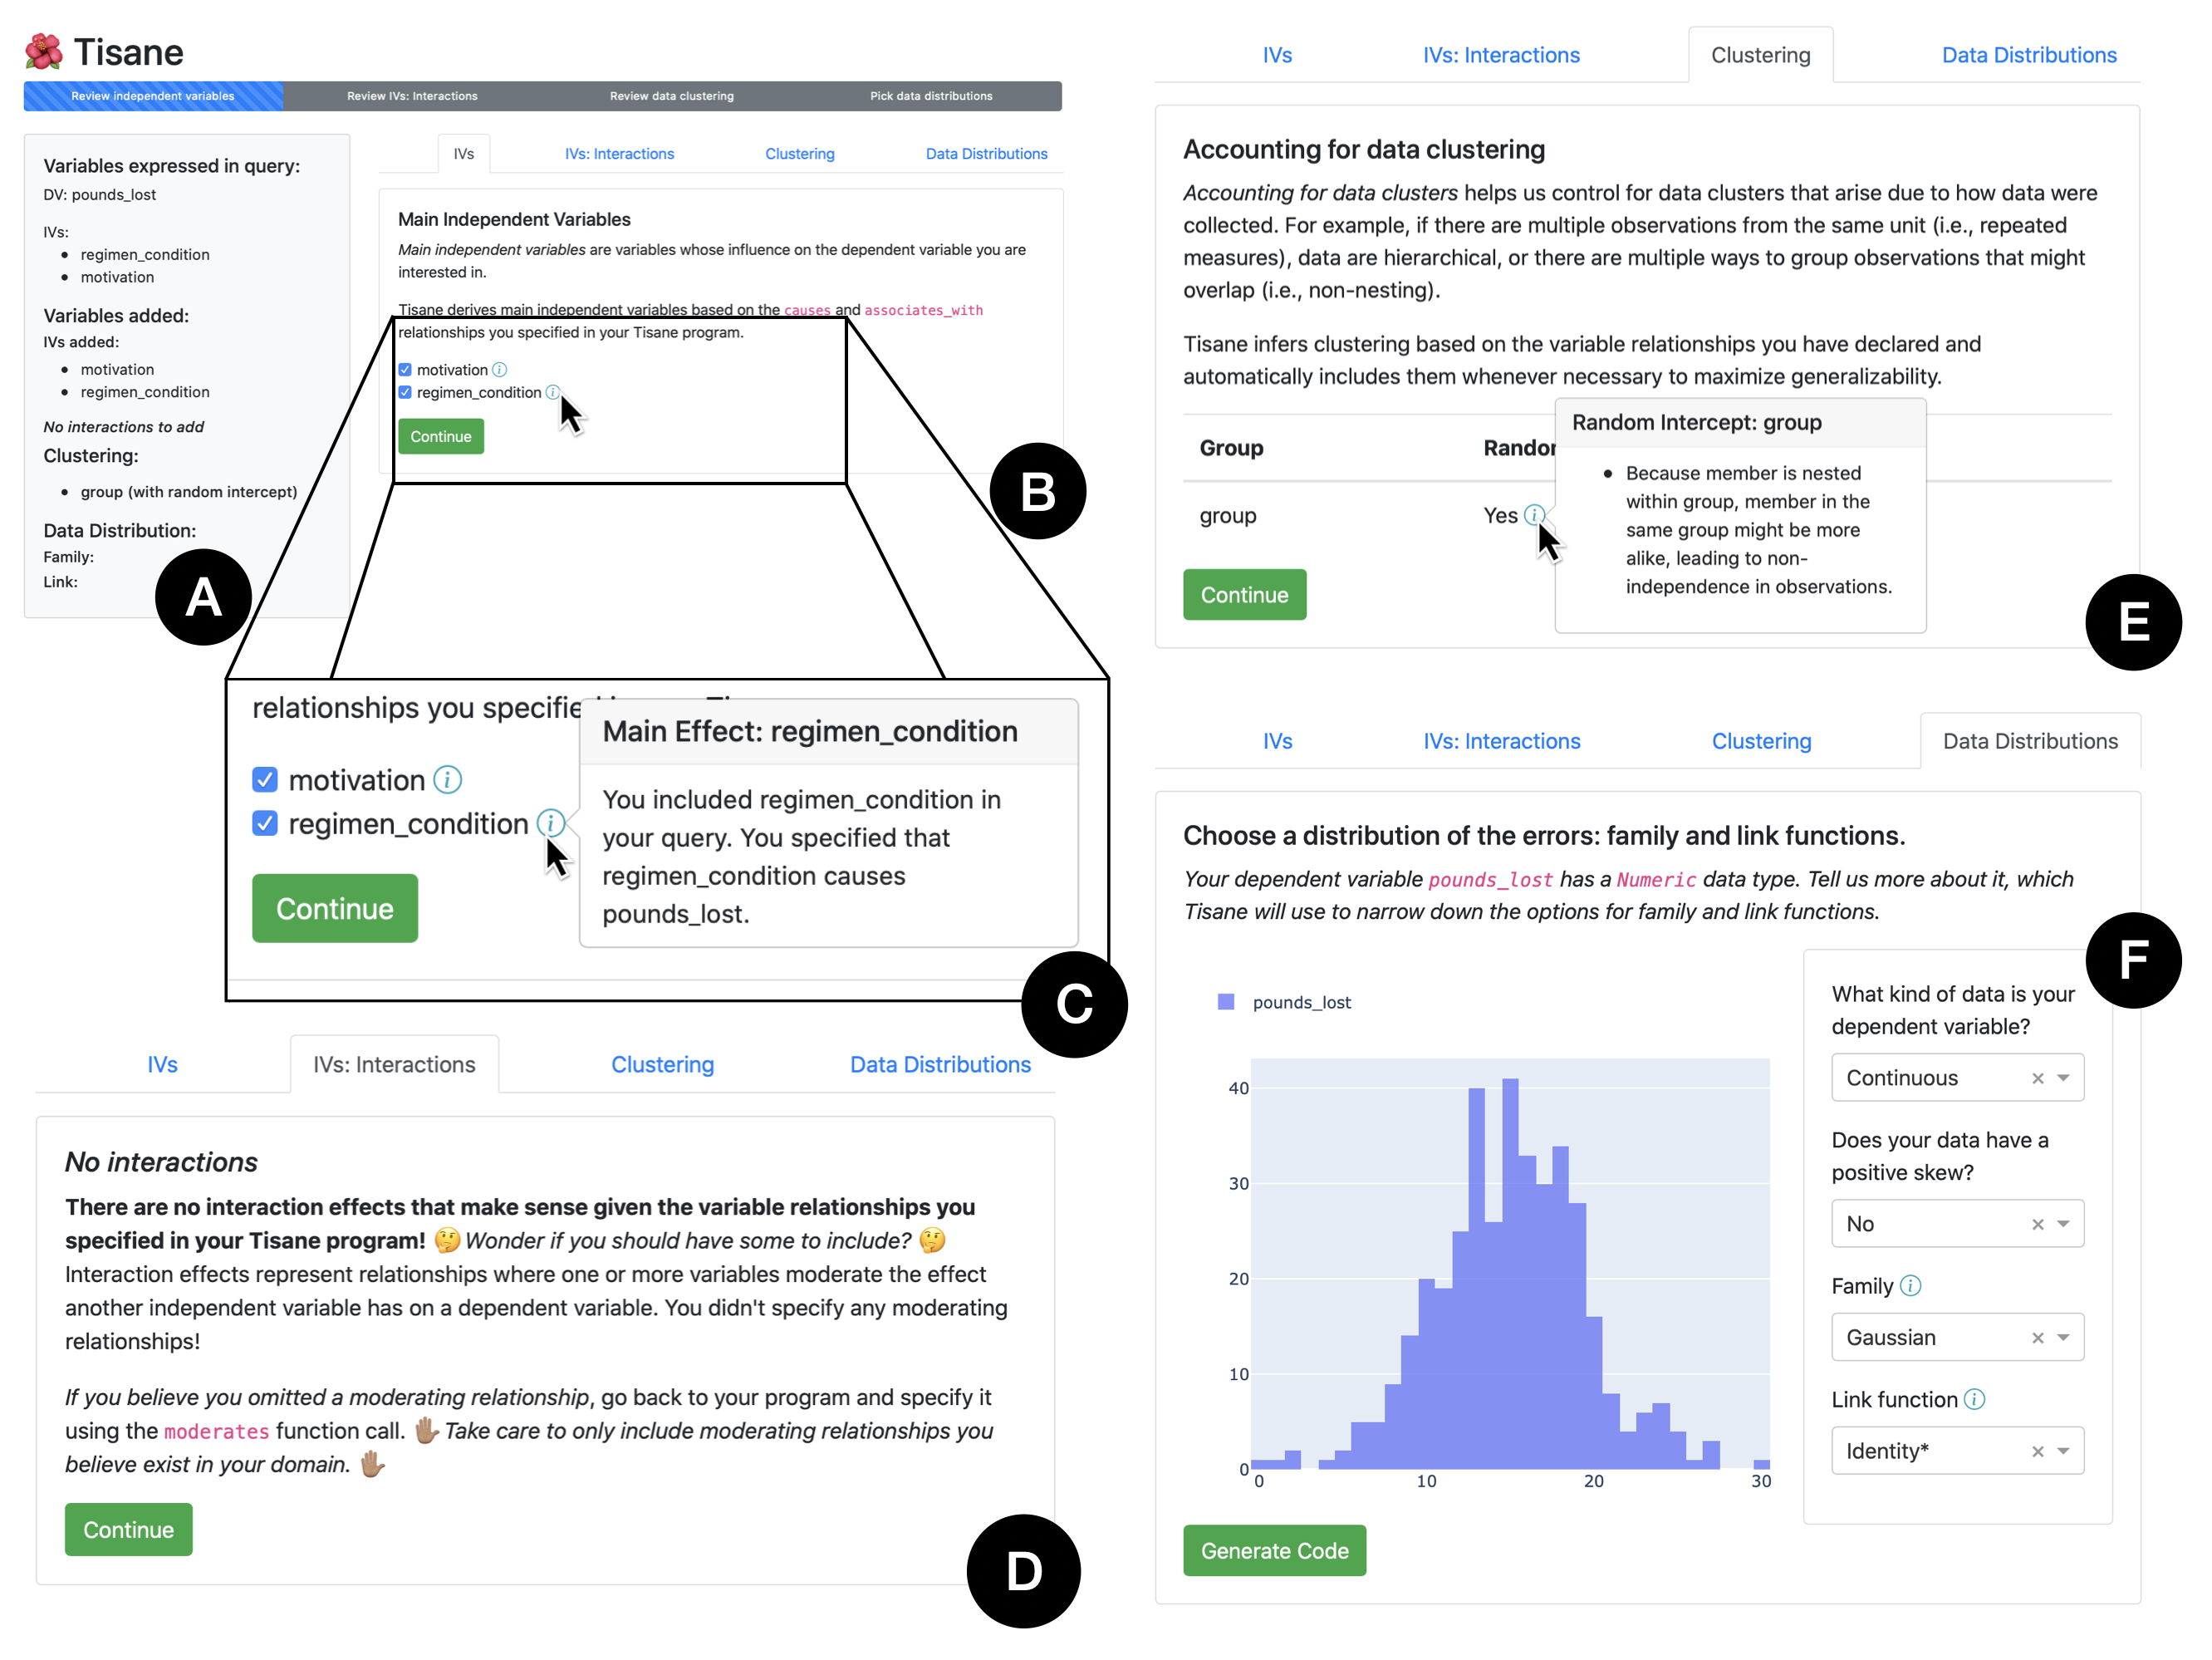
\includegraphics[width=.75\linewidth]{tisane/figures/usage_scenario_gui_05012022.png}
        \caption{Example Tisane GUI for disambiguation. Tisane asks analysts disambiguating questions about variables that are conceptually relevant and that analysts may have overlooked in their query.
        (A) The left hand panel gives an overview of the model the analyst is constructing.
        (B) Based on the variable relationships analysts specify, Tisane infers candidate main effects that may be potential confounders. Tisane asks analysts if they would like to include these variables, explaining in a tooltip
        (C) why the variable may be important to include.
        (D) Tisane only suggests interaction effects if analysts specify moderating relationships in their specification. This way, Tisane ensures that model structures are conceptually justifiable.
        (E) From the data measurement relationships analysts provide, Tisane automatically infers and includes random effects to increase generalizability and external validity of statistical findings.
        (F) Tisane assists analysts in choosing an initial family and link function by asking them a series of questions about their dependent (e.g., Is the variable continuous or about count data?). To help analysts answer these questions and verify their assumptions about the data, Tisane shows a histogram of the dependent variable.
        }
        % (G) \diff{After answering all the disambiguation questions, analysts can generate a script that fits a statistical model and outputs a plot to diagnose the fit of the family function.}
        % }
        % (G) Tisane informs analysts that they should use the histogram to inspect their dependent variable, which may help them select initial family and link functions to try. The normality tests check if the dependent variable is normally distributed, an assumption analysts commonly make but may not apply to their data.}
        % (G) Tisane supports analysts in considering an initia appropriate family and link pair for the final generalized linear model. To help, Tisane provides the results of normality tests and information about how to interpret them.}
        \label{fig:groupExerciseDisambiguation}
        % \Description{Five screenshots of the Tisane GUI are shown. The first screenshot has two labels, (A) and (B), which indicate the overview panel and the main independent variables panel respectively. Above the main effects panel is a series of tabs, which read from left to right: IVs, IVs: Interactions, Clustering, and Data Distributions. The second screenshot, which is labeled (C), shows the result of hovering over one of the info icons in the main independent variables panel, specifically the info icon next to regimen_condition. The tooltip’s body reads: “You included regimen_condition in your query. You specified that regimen_condition causes pounds_lost.” The third screenshot, labeled (D), shows the “IVs: Interactions” tab. It shows the following text, because there were no interaction effects to include in the model: “No interactions  There are no interaction effects that make sense given the variable relationships you specified in your Tisane program! Wonder if you should have some to include? Interaction effects represent relationships where one or more variables moderate the effect another independent variable has on a dependent variable. You didn't specify any moderating relationships! If you believe you omitted a moderating relationship, go back to your program and specify it using the moderates function call. Take care to only include moderating relationships you believe exist in your domain. ” The fourth screenshot, labeled (E), shows the “Clustering” tab. Text at the top of the tab’s panel reads: “Accounting for data clustering  Accounting for data clusters helps us control for data clusters that arise due to how data were collected. For example, if there are multiple observations from the same unit (i.e., repeated measures), data are hierarchical, or there are multiple ways to group observations that might overlap (i.e., non-nesting). Tisane infers clustering based on the variable relationships you have declared and automatically includes them whenever necessary to maximize generalizability.” Below the text is a table. There are two columns. The headers of the columns are “Group” and “Random Intercept.” There is one row beneath the header row, containing “group”, one of the variables in the usage scenario, and “Yes (info-icon)”. A mouse is depicted hovering over the (info-icon) next to “Yes”, and a tooltip has popped up. The header of the tooltip says “Random Intercept: group”. The body of the tooltip gives an explanation for why group was added as a random intercept: “Because member is nested within group, member in the same group might be more alike, leading to non-independence in observations.” Here, member and group are both data variables. The fifth screenshot shows the Data Distributions tab. At the top of the tab’s panel is the title text: “Choose a data distribution: family and link functions. Your dependent variable pounds_lost has a Numeric data type. Tell us more about it, which Tisane will use to narrow down the options for family and link functions.” A right hand panel (F) asks questions about the dependent variable (What kind of data is your dependent variable? Where the option Continuous is selected). To assist, a histogram of the dependent variable is shown. Based on the answers to these questions, Tisane suggests family and link functions. At the very bottom is a “Generate Code” button.}
      \end{figure*}
}

\newcommand{\figurePossibleConfoundingAssociation}{
    \begin{figure}[H]
        \centering
        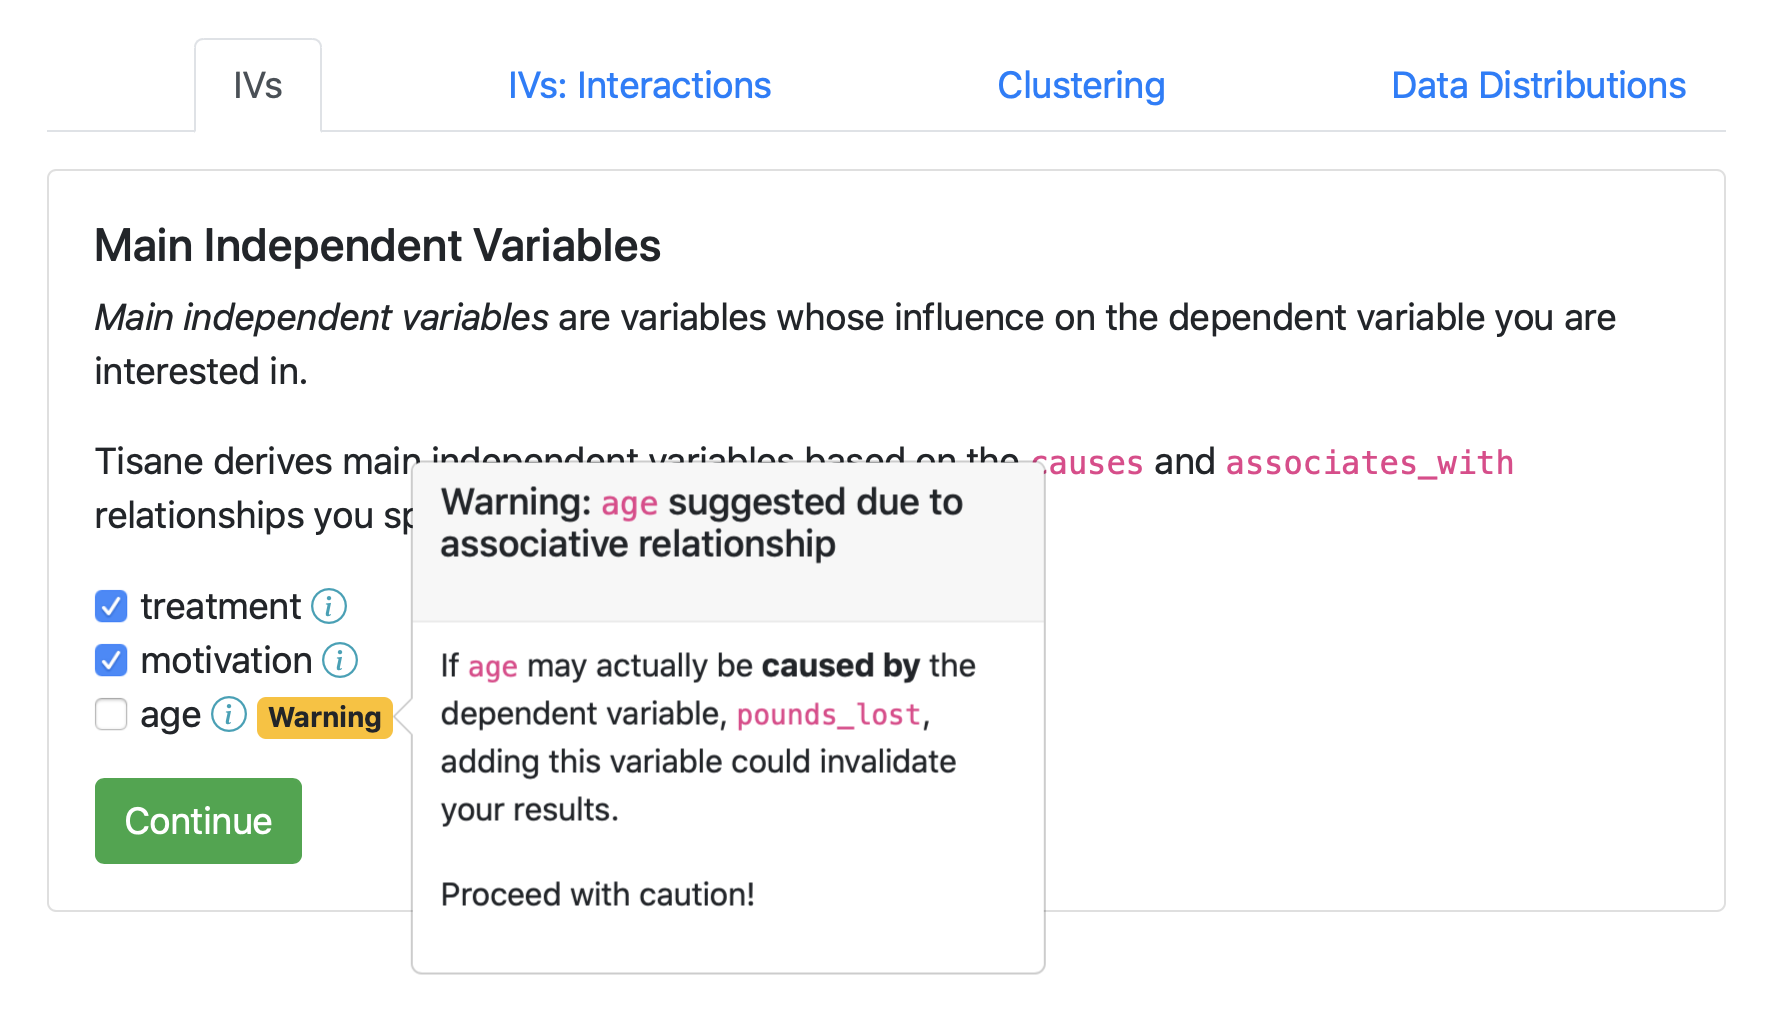
\includegraphics[width=.75\linewidth]{../tisane/figures/tisane_screenshots/potential_confounding_association}
        \caption{An example of the warning text given for potential confounding associations. When analysts hover over the ``Warning'' badge, a tooltip pops up that explains that they should be careful about adding this variable. Associative relationships may in actuality be causal relationships, and if in fact \texttt{pounds\_lost} \textbf{caused} \texttt{age}, then adding \texttt{age} would invalidate the model.}
        \label{fig:figurePossibleConfoundingAssociation}
    \end{figure}
}

\newcommand{\tableStudyDesignTools}{
  \begin{table}
    \small
    \caption{Overview of study design tools that informed Tisane's \SDSLlong.
    The first five tools provide higher-level
    abstractions. They are designed to help researchers reason about their study
    designs more holistically. The latter eight tools are lower-level and are more focused on stimuli,
    trials, and progressions between trials. *JsPsych is the base package to which JsPsychR, xprmtnr, and
    Jaysire provide wrappers and extensions.}
    \begin{tabular}{p{0.25\linewidth}|p{0.75\linewidth}}
      \textbf{Tool}	&	\textbf{Support provided} \\
      \hline
      Edibble~\cite{edibble} 	&	reason about end-to-end experimental design, create data collection schema  \\
      JMP Design of Experiments~\cite{jmpDOE}	&	use templates for experiments, some design optimization, some help with modeling \\
      Gosset~\cite{gosset}	&	search for optimal study design \\
      DeclareDesign~\cite{blair2019declareDesign} 	&	simulate data, specify and reason about designs statistically \\
      Touchstone2~\cite{eiselmayer2019touchstone2}	&	design controlled experiments while reasoning about randomization and statistical power	\\
      Formr~\cite{arslan2020formr}	&	design online survey questions and flow 	\\
      psychTestR~\cite{harrison2020psychtestr}	&	create trials, specify "timelines" for how trials should progress	\\
      Psychopy~\cite{peirce2007psychopy}	&	control how (visual) stimuli are presented, trials, and trial progression in an online experiment	\\
      Psychtoolbox~\cite{borgo2012psychtoolbox}	&	control stimuli in an online experiment, especially for neuroscience 	\\
      JsPysch*~\cite{de2015jspsych} & \multirow{4}{*}{create and control trials and stimuli for online experiments} \\
      JsPyschR~\cite{jspsychR} & \\
      xprmtnr~\cite{xprmntr} & \\
      Jaysire~\cite{jaysire} & \\
    \end{tabular}
    \label{tab:tableStudyDesignTools}
  \end{table}
}


\newcommand{\tableOverallCounts}{
  \begin{table}[ht]
    \begin{tabular}{|p{2cm}|c|c|c|c|c|c|} \hline
                        & \textbf{2017} &\textbf{2018} &\textbf{2019} &\textbf{2020} &\textbf{2021} &\textbf{Total} \\ \hline
      \textbf{repeated}                              &	130	&	168	&	173	&	171	&	163	&	805	\\ \hline
      \textbf{regression}                            &	49	&	66	&	71	&	72	&	72	&	330	\\ \hline
      \textbf{linear model}                          &	9	&	16	&	15	&	12	&	15	&	67	\\ \hline
      \textbf{generalized linear model\footnotemark} &	3	&	1	&	2	&	3	&	0	&	9	\\
      \hline
    \end{tabular}
    \caption{The number of papers from each year, and the total, that contained at least one instance of each of the key words.}
  \end{table}
  \footnotetext{(count is redundant in  ``linear model'')}
}

\newcommand{\tableLinearModelCounts}{
  \begin{table}[ht]
    \begin{tabular}{|l|c|} \hline
                  &	\multicolumn{1}{p{4cm}|}{Number of unique papers that use
                  ``regression'' and/or ``linear model''}	\\ \hline
    \textbf{2017}	&	52	\\ \hline
    \textbf{2018}	&	73	\\ \hline
    \textbf{2019}	&	78	\\ \hline
    \textbf{2020}	&	77	\\ \hline
    \textbf{2021}	&	81	\\ \hline
    \textbf{Total}  &   361 \\ \hline
    \end{tabular}
    \caption{The number of unique papers that contained the key word ``regression'' or ``linear model''.}
    \label{tab:reglmonly}
  \end{table}

}

\newcommand{\tableAnova}{
    \begin{table}
        \caption{Number of papers containing either of the key phrases ``ANOVA'' and ``analysis of variance''.}
        \begin{tabular}{ll} \hline
            \textbf{Year}   &	\textbf{Number of papers} \\ \hline
            2017            &   74 \\
            2018 &              87 \\
            2019 &              89 \\
            2020 &              108 \\
            2021 &              78 \\
            \textbf{Total} &    \textbf{436}
        \end{tabular}
        \label{tab:tableAnova}
    \end{table}
}

\newcommand{\michaelSecondModelOutput}{
    \lstinputlisting[
        language={},
        caption={Output for Michael's second model with pounds lost as the dependent variable and \regimen, \motivation, and \group as independent variables.},
        linerange={1-57},
        label={lst:michaelSecondModelOutput}
    ]{../output/no_interaction_effects.txt}
}

\newcommand{\bridgetModelOutput}{
    \lstinputlisting[
        language={},
        caption={Output for Bridget's model with pounds lost as the dependent variable, \regimen and \motivation as independent variables and \group as a random intercept.},
        linerange={60-81},
        label={lst:bridgetModelOutput}
    ]{../output/no_interaction_effects.txt}
}


\lstset{ %
  language=R,                     % the language of the code
  basicstyle=\footnotesize,       % the size of the fonts that are used for the code
  numbers=left,                   % where to put the line-numbers
  numberstyle=\tiny\color{gray},  % the style that is used for the line-numbers
  stepnumber=1,                   % the step between two line-numbers. If it's 1, each line
                                  % will be numbered
  numbersep=5pt,                  % how far the line-numbers are from the code
  backgroundcolor=\color{white},  % choose the background color. You must add \usepackage{color}
  showspaces=false,               % show spaces adding particular underscores
  showstringspaces=false,         % underline spaces within strings
  showtabs=false,                 % show tabs within strings adding particular underscores
%   frame=single,                   % adds a frame around the code
  rulecolor=\color{black},        % if not set, the frame-color may be changed on line-breaks within not-black text (e.g. commens (green here))
  tabsize=2,                      % sets default tabsize to 2 spaces
  captionpos=b,                   % sets the caption-position to bottom
  breaklines=true,                % sets automatic line breaking
  breakatwhitespace=false,        % sets if automatic breaks should only happen at whitespace
  title=\lstname,                 % show the filename of files included with \lstinputlisting;
                                  % also try caption instead of title
  keywordstyle=\color{blue},      % keyword style
  commentstyle=\color{dkgreen},   % comment style
  stringstyle=\color{mauve},      % string literal style
  escapeinside={\%*}{*)},         % if you want to add a comment within your code
  morekeywords={*,...}            % if you want to add more keywords to the set
} 

\newcommand{\rTisaneProgram}{
    \lstinputlisting[
        language={}, 
        caption={Sample \rTisane program.},
        label={lst:rTisaneProgram}
    ]{tisane/figures/rTisane-example.R}
}